\chapter[Code demonstration and validation]{Code demonstration and validation}

After refactoring, redesign, and implementation of the new capabilities 
mentioned in Chapter 3, SaltProc v1.0 will be tested for the \gls{TAP} 
\gls{MSR}. The \gls{TAP} concept was selected because it is well analyzed in 
the literature\cite{betzler_two-dimensional_2017, betzler_assessment_2017}; 
thus, cross-code verification with ChemTRITON/SCALE is possible 
\cite{betzler_assessment_2017}. The demonstration will be performed for two 
timescales:
\paragraph{Long-term.} The reactor lifetime-long (e.g., 40 years) depletion 
simulation will be performed with moderate time resolution (e.g., 30-day 
depletion step). The results obtained with SaltProc v1.0 will be compared 
with recent efforts discussed in Chapter 2, more specifically with Betzler 
\emph{et al.}  \cite{betzler_assessment_2017}. That validation effort will 
help to ensure that SaltProc v1.0 solution is correct for the case with ideal 
extraction efficiency.
\paragraph{Short-term (transient).} The 7-day-long depletion simulation with 
changing, load following core power will be performed with the fine time 
resolution (e.g., 5-min depletion step). The depletion calculation for the 
\gls{TAP} in load following regime would capture the effects of xenon 
poisoning and evaluate the benefit of using an online gas removal system.

Additionally, a compatible \textit{.json} database with input examples of 
various fuel reprocessing system configurations for use with SaltProc v1.0 
will be released to encourage research efforts in online reprocessing 
simulations for various \gls{MSR} designs.

\section{Transatomic Power Molten Salt Reactor concept}
The \gls{TAP} concept is a 1250 MW$_{th}$ \gls{MSR} with a LiF-based uranium 
fuel salt \cite{transatomic_power_corporation_technical_2016}. This concept 
uses configurable zirconium hydride rods as the moderator while most \gls{MSR} 
designs typically propose high-density reactor graphite. Zirconium hydride 
offers a much higher neutron moderating density than graphite: much less 
zirconium hydride volume is needed to achieve a thermal energy spectrum 
similar to one obtained with graphite moderator. Moreover, zirconium hydride 
has a much longer lifespan in extreme operational conditions (high 
temperature, large neutron flux, chemically aggressive salt) than reactor 
graphite. Finally, zirconium hydride is a nonporous material and holds up 
fewer neutron poisons (e.g., xenon, krypton) than does high-density 
reactor graphite.

In this section, the design characteristics and reprocessing plant design are 
based on
information presented in the TAP white papers  
\cite{transatomic_power_corporation_technical_2016, 
transatomic_power_corporation_neutronics_2016} and \gls{ORNL} technical 
reports \cite{betzler_two-dimensional_2017, betzler_assessment_2017}.

\subsection{TAP design description}
\begin{figure}[h] % replace 't' with 'b' to 
	  		\hspace{+2.2in}
	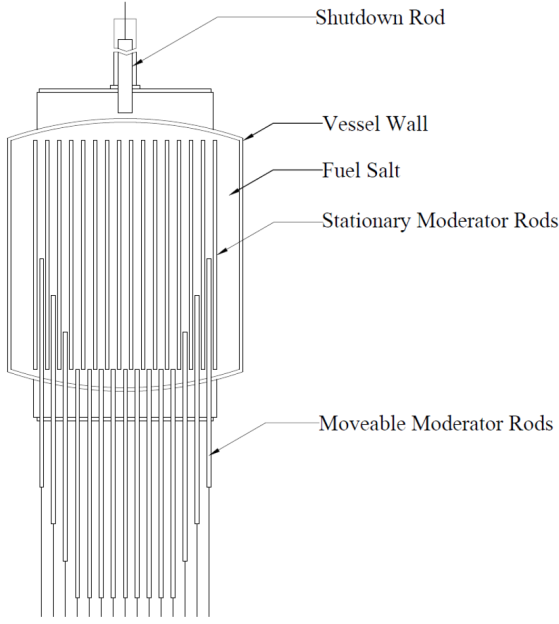
\includegraphics[width=0.65\textwidth]{tap_front_view.png}
	\caption{The \gls{TAP} \gls{MSR} schematic view showing movable moderator 
		rod 
		bundles and shutdown rod (figure reproduced from Transatomic Power 
		White Paper 
		\cite{transatomic_power_corporation_technical_2016}).}
	\label{fig:tap-main-view}
\end{figure}
The \gls{TAP} design (figure~\ref{fig:tap-main-view}) is very similar to 
original \gls{MSRE} design developed by \gls{ORNL} 
\cite{haubenreich_experience_1970} but has two major innovations: 
the fuel salt composition and the moderator. The \gls{MSRE}'s 
LiF-BeF$_2$-ZrF$_4$-UF$_4$ salt has been substituted with LiF-UF$_4$ salt 
which allows for an increase in the uranium concentration within the fuel salt 
from 0.9 to 27.5\% while maintaining a relatively low melting point 
(490$^{\circ}$C compared with 434$^{\circ}$C for the original \gls{MSRE}'s 
salt) \cite{betzler_two-dimensional_2017}. The graphite has a very high 
thermal scattering cross section which makes it a perfect moderator but has 
a few major drawbacks: 
(1) the low lethargy gain per collision requires a large volume of moderator 
to be present to reach criticality, which leads to a larger core and obstructs 
the core power density; (2) even special 
reactor-grade graphite has relatively high porosity, consequently, it holds
gaseous \glspl{FP} 
(e.g., tritium, xenon) in pores; (3) the reactor graphite lifespan in a 
commercial 
reactor is approximately 10 years \cite{robertson_conceptual_1971}. As previously 
mentioned, to resolve these issues, the \gls{TAP} concept uses zirconium 
hydride instead, allowing for a more compact core and a significant increase 
in power density. These two innovative design choices, together with a 
configurable moderator (the moderator-to-fuel ratio can be changed during 
regular maintenance shutdown), facilitate the deployment of this conceptual 
design in the current commercially available 5\% enriched \gls{LEU} fuel cycle. 

The \gls{TAP} \gls{MSR} primary loop contains the reactor core volume 
(including the zirconium hydride moderator rods with silicon carbide 
cladding), pumps, and primary heat exchanger. Pumps circulate the 
LiF-(Act)F$_4$ fuel salt through the primary loop. The pumps, vessels, tanks, 
and piping are made of a nickel-based alloy (similar to Hastelloy-N\footnote{ 
Hastelloy-N is very common in \gls{MSR} concepts now, having been
developed at \gls{ORNL} in the \gls{MSRE} program that started in the 
1950s.}), which is highly resistant to corrosion in various molten salt 
environments. Inside the reactor vessel, near the zirconium hydride moderator 
rods, the fuel salt is in a critical configuration and generates heat. 
Table~\ref{tab:tap_tab} contains details of the \gls{TAP} system design which 
are taken from technical white paper 
\cite{transatomic_power_corporation_technical_2016} and a neutronics overview 
\cite{transatomic_power_corporation_neutronics_2016} as well as \gls{ORNL} 
analysis of the \gls{TAP} design \cite{betzler_two-dimensional_2017, 
betzler_assessment_2017}. 
%%%%%%%%%%%%%%%%%%%%%%%%%%%%%%%%%%%%%%%%
\begin{table}[h!]
	\caption{Summary of principal data for the \gls{TAP} \gls{MSR} 
		(reproduced from \cite{transatomic_power_corporation_technical_2016, 
		betzler_assessment_2017}). }
	\begin{tabularx}{\textwidth}{ s  s}
		\hline
		Thermal power				           		& 1250 MW$_{th}  $       
		\\ 
		Electric power		                		& 520 MW$_e  $ 			 
		\\ 
		Gross thermal efficiency        			& 44\%     				 
		\\  
		Outlet temperature							& 620$^{\circ}$C         
		\\ 
		Fuel salt components                   & LiF-UF$_4$				 \\  
		Fuel salt composition                  & 72.5-27.5 mole\%			 
		\\  
		Uranium enrichment                     & 5\% $^{235}$U          	 \\
		Moderator                              & Zirconium Hydride 
		(ZrH$_{1.66}$) rods (with silicon carbide cladding) \\
		Neutron spectrum						& 
		thermal/epithermal                 \\
		\hline
	\end{tabularx}
	\label{tab:tap_tab}
\end{table}
%%%%%%%%%%%%%%%%%%%%%%%%%%%%%%%%%%%%%%%%%%%%%%%%
\subsection{TAP core design}
In the \gls{TAP} core (figure~\ref{fig:tap-core-view}), fuel salt flows around 
moderator assemblies consisting of lattices of zirconium hydride rods clad in 
a corrosion-resistant silicone carbide (figure~\ref{fig:tap-main-view}). The 
\gls{TAP} reactor pressure vessel is a cylinder with an inner radius 150 cm, 
height 350 cm, and wall thickness 5 cm made of a nickel-based alloy. 
\begin{figure}[t] % replace 't' with 'b' to 
	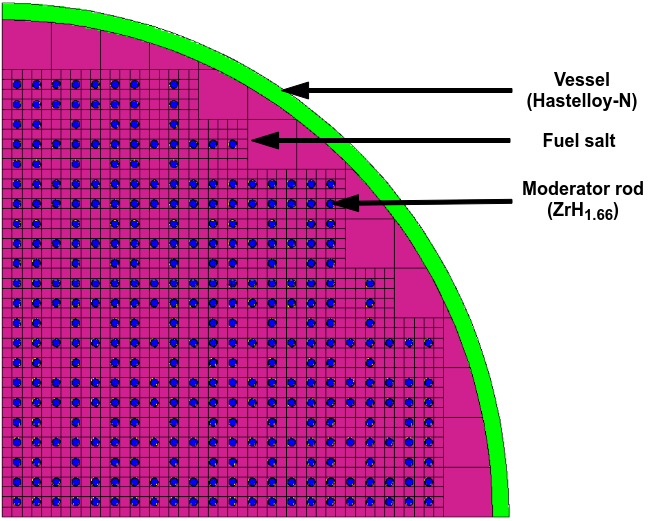
\includegraphics[width=\textwidth]{tap_core_ornl.png}
	\vspace{-0.35in}
	\caption{The \gls{TAP} \gls{MSR} schematic core view showing moderator 
		rods 
		(figure reproduced from ORNL/TM-2017/475  
		\cite{betzler_assessment_2017}).}
	\label{fig:tap-core-view}
\end{figure}

The \gls{SVF} in the core is parameter similar to wide-used moderator-to-fuel 
ratio and can be defined as:
\begin{align}
SVF &= \frac{V_F}{V_F+V_M} = \frac{1}{1+V_M/V_F}
\intertext{where}
V_F &= \mbox{the fuel volume} \nonumber \\
V_M &= \mbox{the moderator volume} \nonumber \\
V_M/V_F &= \mbox{the moderator-to-fuel salt ratio.} \nonumber
\end{align}

The \gls{SVF} in the core can be varied during operation to shift the 
spectrum from intermediate to thermal energies (from \gls{BOL} to \gls{EOL}, 
respectively) to maximize fuel burnup. In practice, \gls{SVF} can be varied by 
inserting fixed-sized moderator rods via the bottom of the reactor vessel (for 
safety considerations), similarly to moving the control rods in a \gls{BWR}, 
as shown in Figure~\ref{fig:tap-main-view}. For the \gls{TAP} reactor, 
\gls{EOL} occurs when the maximum number of moderator rods are inserted into 
the core, and a further injection of fresh fuel salt does not alter
criticality. Unmoderated salt is flowing in the annulus between the core, and 
the vessel wall provides for a potential reduction in fast neutron flux at the 
vessel structural material  
\cite{transatomic_power_corporation_neutronics_2016}.

\subsection{Serpent 2 full-core model} \label{sec:tap_model}
Nest and lattice geometry types as well as universe transformation 
capabilities of Serpent \cite{leppanen_serpent_2013} are employed to represent 
\gls{TAP} core. Figure~\ref{fig:tap-serpent-plan} shows the $XY$ section of 
whole-core
configuration at the expected reactor operational level when all
control rods are fully withdrawn. Figures~\ref{fig:tap-serpent-elev} and 
~\ref{fig:tap-serpent-elev-zoom} show a longitudinal section of the reactor. 
This model contains the moderator rods with silicon carbide cladding, pressure 
vessel, and inlet and outlet plena (Table~\ref{tab:tap_model_param}). Fuel 
salt flows around rectangular moderator assemblies consisting of lattices of 
small-diameter zirconium hydride rods in a corrosion-resistant material. The 
\gls{SVF} for model herein is 0.907268, which means the modeled core is 
under-moderated and has an intermediate, epithermal spectrum.
\begin{figure}[htp!] % replace 't' with 'b' to 
	\centering
	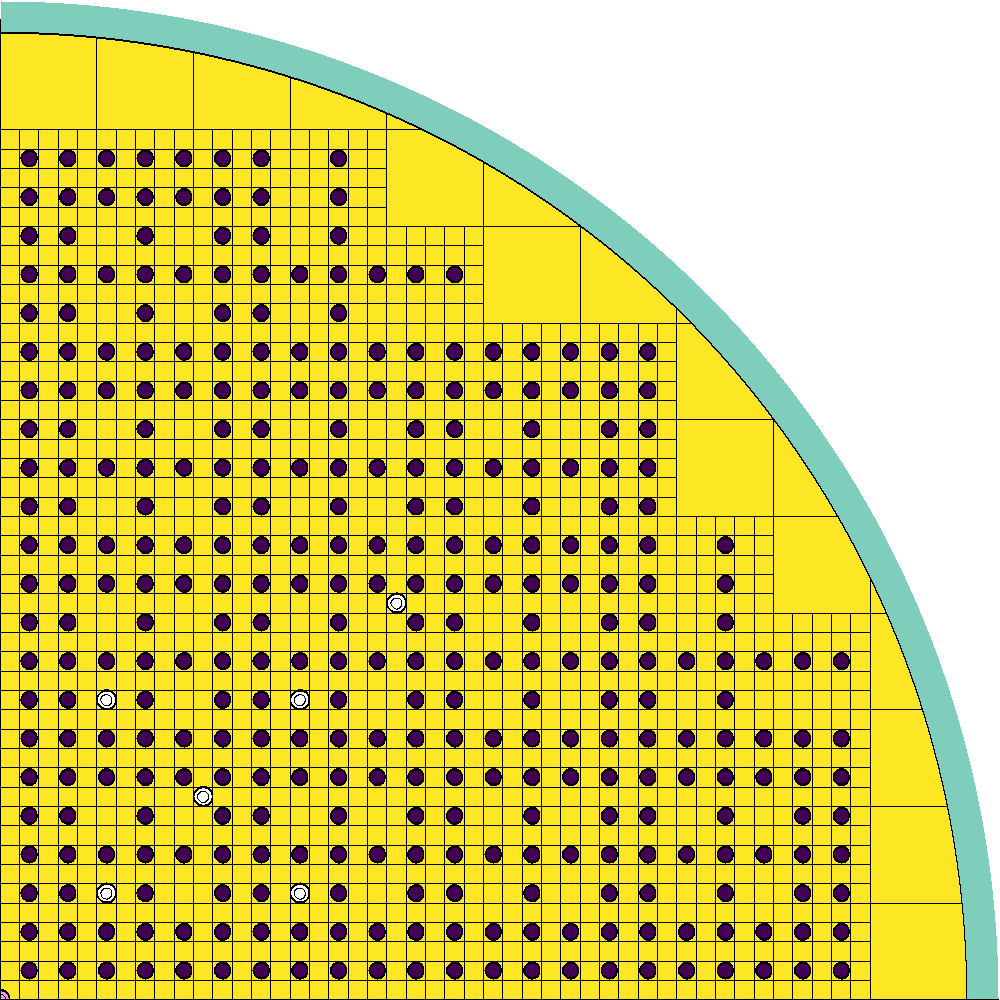
\includegraphics[width=0.95\textwidth]{tap_plan_view.png}
	\caption{An $XY$ section of the \gls{TAP} model at horizontal midplane 
		with fully withdrawn control rods at \gls{BOL} (\gls{SVF}$=0.907268$). 
		The violet color represents zirconium 
		hydride, and the yellow represents fuel salt. The blue color shows 
		Hastelloy-N, a material used for the vessel wall, and the white color 
		is the air.}
	\label{fig:tap-serpent-plan}
\end{figure}
\begin{figure}[htp!] % replace 't' with 'b' to 
	\centering
	
\includegraphics[width=\textwidth]{tap_elev_view.png}
	\caption{An $XZ$ section of the \gls{TAP} model.}
	\label{fig:tap-serpent-elev}
\end{figure}
\begin{figure}[htp!] % replace 't' with 'b' to 
	\centering
	\includegraphics[width=0.4\textwidth]{tap_elev_view_zoomed.png}
	\caption{Zoomed $XZ$ section of the top of the moderator rods and guide 
	tubes in the \gls{TAP} model. The orange color shows 70-30\%  
	Gd$_2$O$_3$-Al$_2$O$_3$ ceramic absorbers used for control rods.}
	\label{fig:tap-serpent-elev-zoom}
\end{figure}

To represent the reactivity control system, the model has: (1) control rod 
guide tubes made of nickel-based alloy; (2) control rods represented as hollow 
70-30\% Gd$_2$O$_3$-Al$_2$O$_3$ cylinders with a thin Hastelloy-N coating 
\cite{betzler_assessment_2017}; (3) air inside guide tubes and control rods. 
The control rod design is comprised of a cluster of 25 rods that provide a 
total reactivity worth of $1110\pm9.7pcm$.
%%%%%%%%%%%%%%%%%%%%%%%%%%%%%%%%%%%%%%%%%%%%%%%%%%
\begin{table}[hb!]
	\caption{Geometric parameters for the full-core 3D model of the 
		\gls{TAP} (reproduced from Betzler \emph{et al.} 
		\cite{betzler_assessment_2017}). }
	\centering
	\begin{tabularx}{0.9\textwidth}{s s x p{0.14\textwidth}}
		\hline
		\textbf{Component}&\textbf{Parameter}&\textbf{Value}& \textbf{Unit}   
		\\ \hline
		\multirow{4}{*}{\begin{tabular}[c]{@{}l@{}}Moderator\\ 
				rod\end{tabular}} 
		& Cladding thickness      	  			    & 0.10 & cm				 
		\\  
		& Radius 				      	  			& 1.15 & cm				 
		\\  
		& Length				      	  			& 3.0  & m				 
		\\  
		& Pitch				      	  			& 3.0  & cm  			 \\ 
		\hline 
		
		\multirow{2}{*}{\begin{tabular}[c]{@{}l@{}}Moderator\\ 
				assembly\end{tabular}} 
		& Array				      	  			& 5 $\times$ 5 & 
		rods$\times$rods \\  
		& Pitch				      	  			& 15.0 & cm    				 
		\\  \hline
		
		\multirow{4}{*}{\begin{tabular}[c]{@{}l@{}}Core\end{tabular}}          
		& Assemblies  				   	  			& 268  & assemblies/core 
		\\  
		& Inner radius			      	  			& 1.5  & 
		m    				 \\  
		& Plenum height			   	  			& 25.0 & cm    				 
		\\  
		& Vessel wall thickness     	  			& 5.0 & 
		cm    				 \\ \hline            
	\end{tabularx}
	\label{tab:tap_model_param}
\end{table}
%%%%%%%%%%%%%%%%%%%%%%%%%%%%%%%%%%%%%%%%%%%%%%%%

The control rod cluster is modeled using the \textbf{TRANS} Serpent 2 feature, 
which allows the user to easily change the control rod position during the 
simulation. Herein I assumed that all control rods are fully withdrawn from 
the core (figure~\ref{fig:tap-serpent-elev-zoom}), but control rod 
positions may vary in future investigations.
In this report, all figures of 
the core were generated using the built-in Serpent plotter.

\section{TAP fuel salt reprocessing system}
The \gls{TAP} nuclear island contains the \gls{FP} removal system. Gaseous  
\glspl{FP} are continuously removed using an off-gas system while liquid and 
solid \glspl{FP} are extracted via a chemical processing system. As these 
byproducts are gradually removed, a small quantity of fresh fuel salt is 
regularly added to the primary loop. This process conserves a constant fuel 
salt mass and keeps the reactor critical. In contrast with the \gls{MSBR} 
reprocessing system, the \gls{TAP} design does not need a protactinium 
separation and isolation system because it operates in a uranium-based 
single-stage fuel cycle. The authors of the \gls{TAP} concept suggested three 
distinct fission product removal methods 
\cite{transatomic_power_corporation_neutronics_2016}:
\paragraph{Off-Gas System:} The off-gas system removes gaseous fission 
products such as krypton and xenon, which are then compressed and stored 
temporarily until they have decayed to the background radiation level. Trace 
amounts of tritium are also removed and bottled in a liquid form via the same 
process. Also, the off-gas system directly removes a small fraction of the 
noble metals.
\paragraph{Metal Plate-Out/Filtration:} A nickel mesh filter removes noble and 
semi-noble metal solid fission products as they plate out onto internal surface
of the filter.
\paragraph{Liquid Metal Extraction:} Lanthanides and other non-noble metals 
stay dissolved in the fuel salt. They generally have a lower capture cross 
section and thus absorb fewer neutrons than $^{135}$Xe, but their extraction 
is essential to ensure normal operation. In the \gls{TAP} reactor, lanthanide 
removal is accomplished via a liquid-metal/molten salt extraction process 
similar to that developed for \gls{MSBR} by \gls{ORNL}  
\cite{robertson_conceptual_1971}. The process converts the dissolved 
lanthanides into a well-understood oxide waste form, similar to that of 
\gls{LWR} \gls{SNF}. This oxide waste comes out of the \gls{TAP} reprocessing 
plant in ceramic granules and can be sintered into another convenient form for 
storage \cite{transatomic_power_corporation_technical_2016}.

Figure~\ref{fig:tap-reproc} shows the principal design of the \gls{TAP} 
primary loop, including an off-gas system, nickel mesh filter, and lanthanide 
chemical extraction facility. Similarly to the \gls{MSBR}, an off-gas system 
is also based on a simple process of helium sparging through fuel salt with 
consequent gas bubbles removed before returning the fuel salt to the core. 
Nevertheless, one crucial difference must be noted: the \gls{MSBR} gas 
separation system suggested helium injection and subsequent transport of the 
voids throughout the primary loop, including the core for at least ten full 
loops \cite{robertson_conceptual_1971}. It is a significant concern to safe, 
stable operation because the increase of void fraction in the fuel salt when 
it enters back to the core would cause unpredictable reactivity change. This 
drawback can be overcome by using an effective gas separator for stripping 
helium/xenon bubbles before returning the salt to a primary loop 
(Figure~\ref{fig:tap-reproc}, blue block). 
\begin{figure}[htp!] % replace 't' with 'b' to 
	\centering
	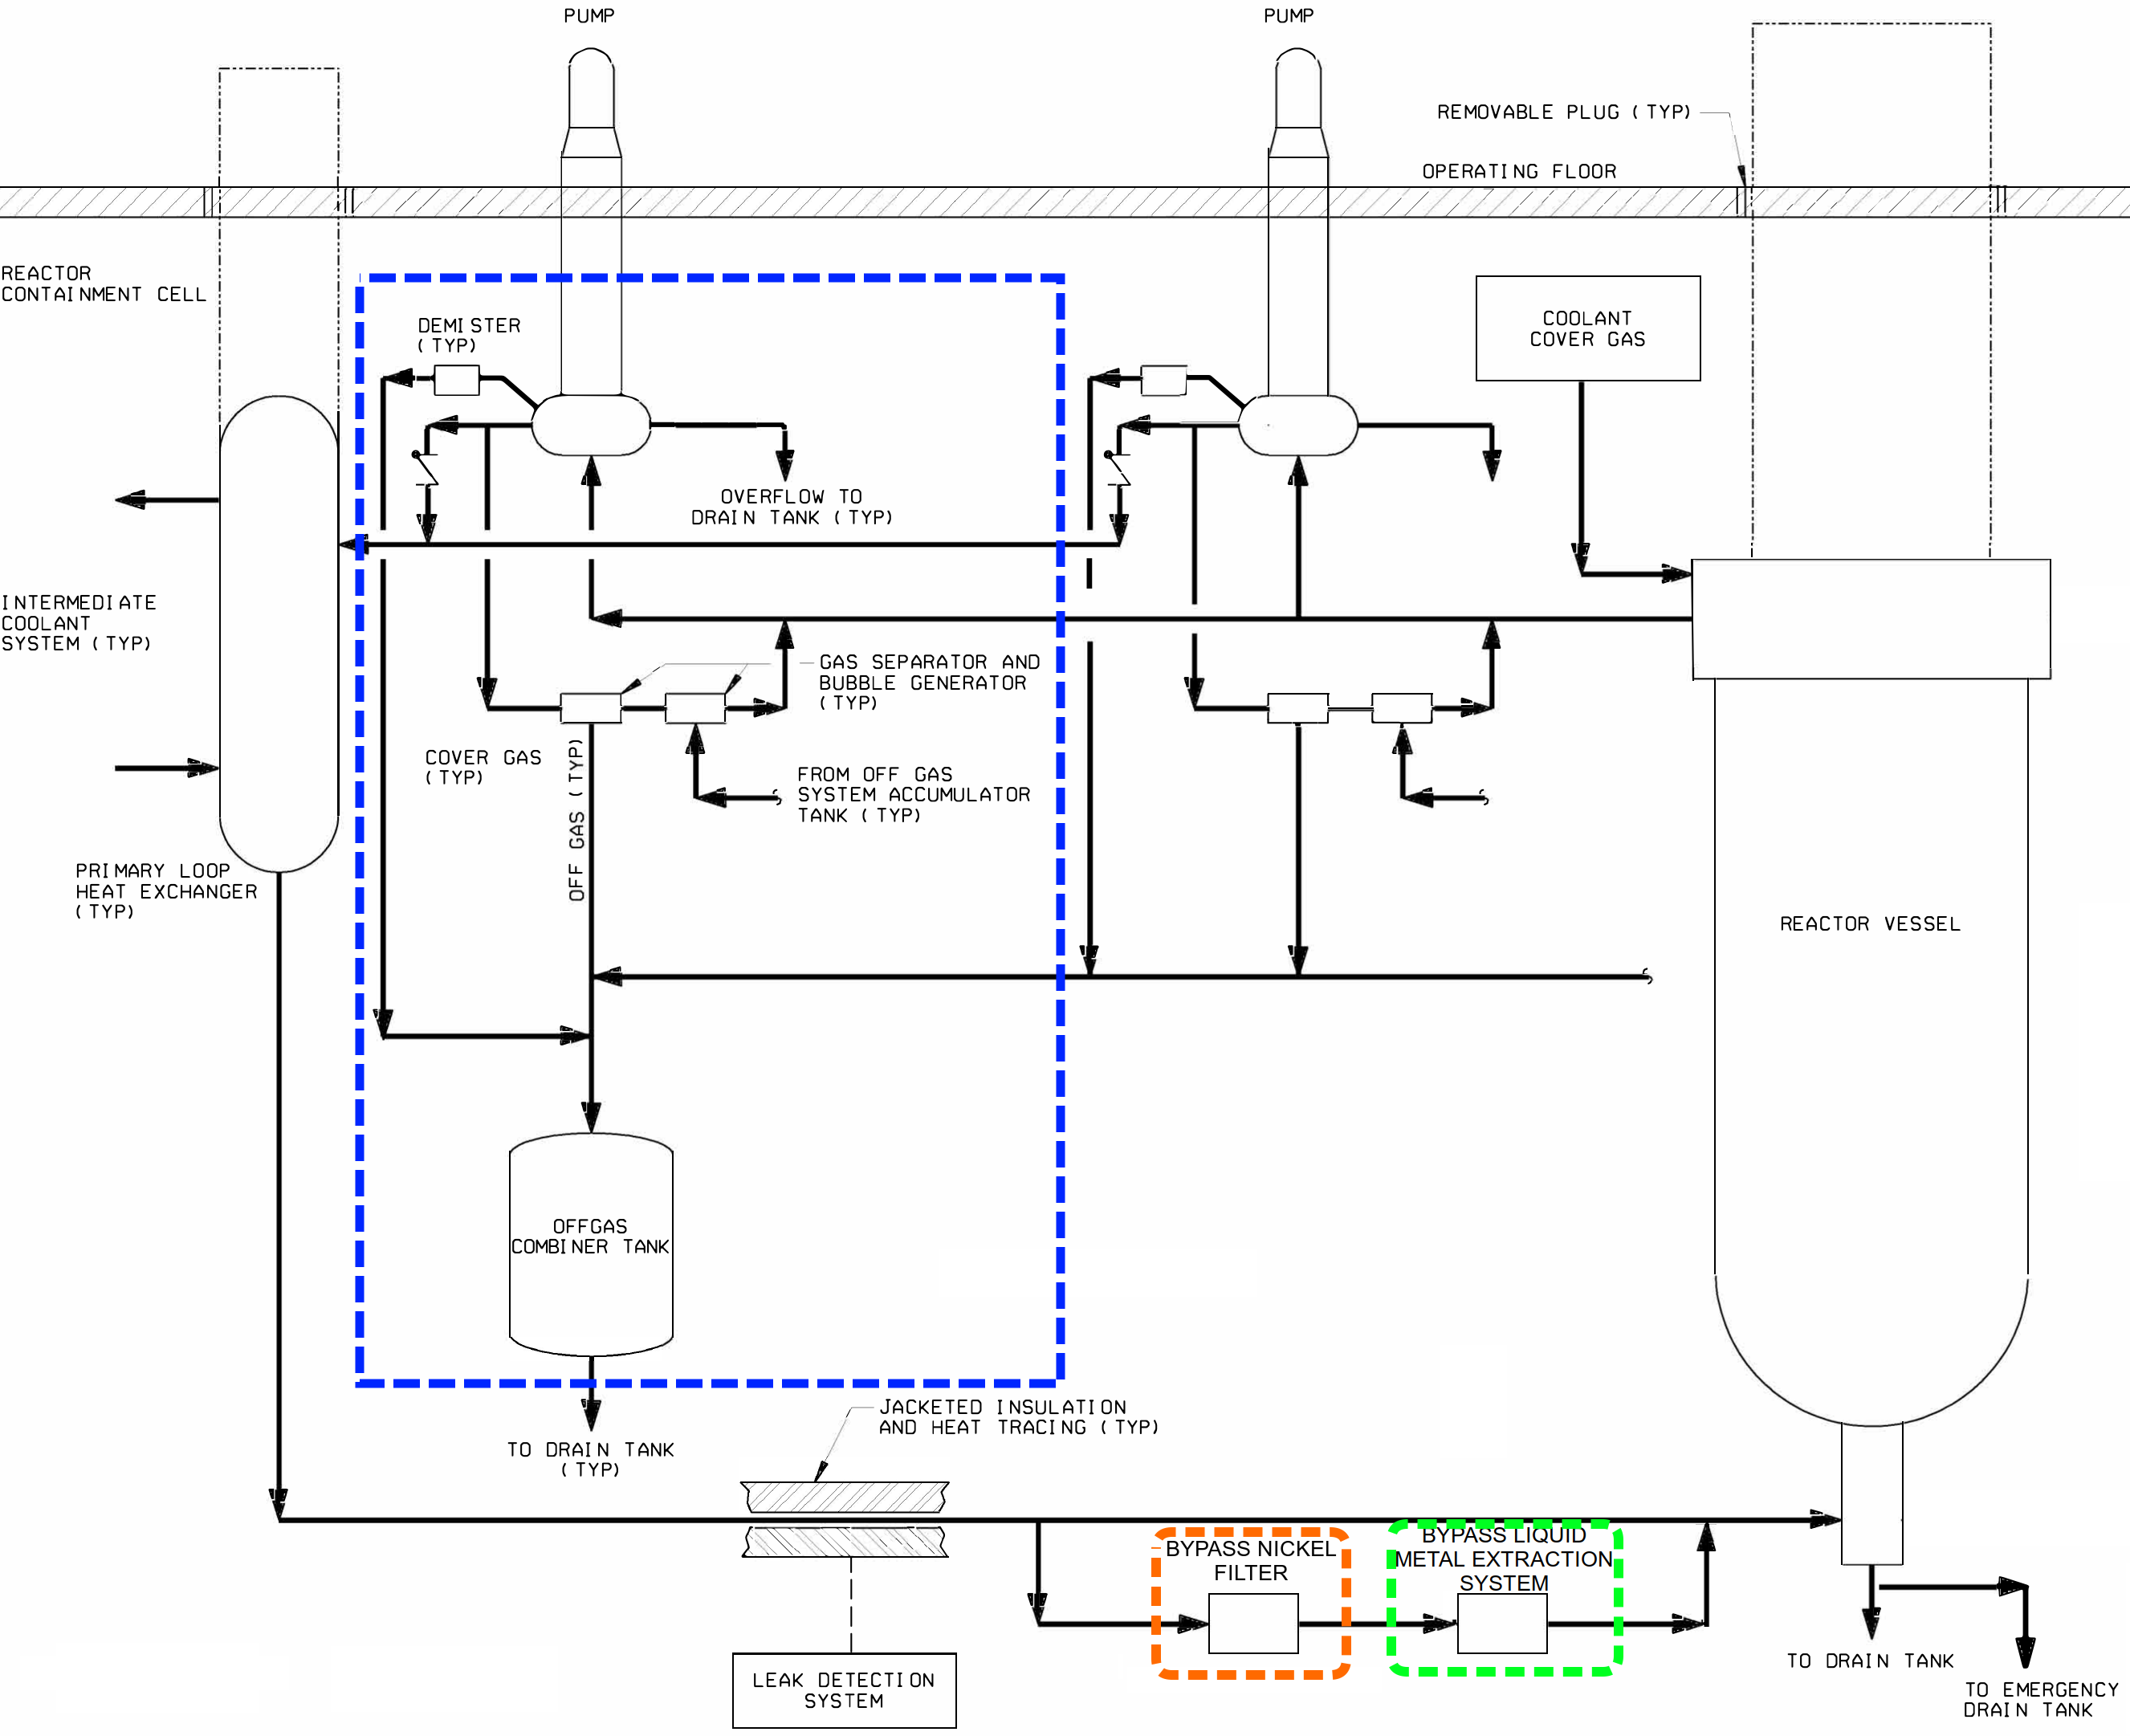
\includegraphics[width=\textwidth]{tap_primary_loop.png}
	\caption{Simplified \gls{TAP} primary loop design including off-gas system 
	(blue), 
		nickel filter (orange) and liquid metal extraction system (green) 
		(reproduced from \cite{transatomic_power_transatomic_2019}).}
	\label{fig:tap-reproc}
\end{figure}

Noble and semi-noble metal solid fission products tend to plate out onto metal 
surfaces including piping, heat exchanger tubes, reactor vessel inner surface, 
etc. Previous research by \gls{ORNL} \cite{robertson_conceptual_1971} reported 
that about 50\% of noble and semi-noble metals would plate out inside 
\gls{MSBR} systems without any special treatment. To improve the extraction 
efficiency of these fission products, the \gls{TAP} concept suggested 
employing a nickel mesh filter located in a bypass stream in the primary loop 
(Figure~\ref{fig:tap-reproc}, orange block). The main idea of this filter is 
to create a maze with large metal (nickel) surface area. The fuel salt is  
flowing throughout the filter and noble metals plate-out on the internal  
filter surface. 

This Liquid Metal Extraction process for the \gls{TAP} concept has been 
adopted from the \gls{MSBR}. The \gls{MSRE} demonstrated a liquid-liquid 
extraction process for removing rare earths and lanthanides from fuel salt and 
estimated efficiency of this process. Removal efficiency ($\epsilon_{RE}$) of  
this process is the function of salt mass flow rate, liquid bismuth mass 
flow rate, interfacial areas between salt and metal, and mass transfer 
coefficient for each noble metal species. The most recent research for LiF 
salt (for the \gls{MSFR} concept) reported the following form of extraction 
efficiency correlation \cite{rodrigues_actinide/lanthanide_2015}:
\begin{align} 
\epsilon_{RE} &= \frac{1}{1+10^{\lambda}} \nonumber \\
&= \frac{1}{1+10^{f(A, \dot{m}_{Bi}, \dot{m}_{salt}, N, K)}} \label{eq:re_eff}
\intertext{where}
A&= \mbox{metal-to-salt interface area} \nonumber \\
\dot{m}_{Bi}&= \mbox{bismuth mass flow rate} \nonumber \\
\dot{m}_{salt}&= \mbox{salt mass flow rate} \nonumber \\
N&= \mbox{number of stages} \nonumber \\
K&= \mbox{liquid phase mass transfer coefficient} \nonumber 
\end{align}
Correlations are different for various lanthanides and can be determined from 
experimental data and/or existing analytical models 
\cite{mcneese_engineering_1971, delpech_possible_2012, 
rodrigues_actinide/lanthanide_2015}.

In fact, due to similarities in reprocessing schemes, the \gls{TAP} project 
reported almost the same set of elements for removal and similar effective 
cycle times as suggested for \gls{MSBR} (Table~\ref{tab:reprocessing_list}). 
The \gls{TAP} neutronics whitepaper specifies additional low-probability 
fission products and gases that should be removed during operation. These 
elements are categorized into the previously defined processing groups, but 
the removal rates of most of these elements (i.e., all except for hydrogen) 
are very low.

Details of gas removal and fuel reprocessing systems have historically 
been conceptual. Accordingly, liquid-fueled system designs including the 
\gls{TAP} concept usually assume ideal (rather than realistically constrained) 
removal efficiencies for reactor performance simulations. For the proposed 
work, a realistic online reprocessing system and reactor model will be created 
to capture the dynamics of fuel composition evolution during reactor 
operation. Gas removal efficiency will be represented in that model as a 
variable, described using mathematical correlation from Chapter 2 (see  
Equation~\ref{eq:gas_eff}). For the other \glspl{FP}, a fixed\footnote{ 
Published information about dynamics of extraction efficiency during reactor 
operation for seminoble metals, volatile fluorides, and rare earths is 
insufficient to inform a variable removal efficiency.}, non-ideal 
extraction efficiency based on cycle time from 
Table~\ref{tab:reprocessing_list} will be used in the fuel reprocessing model.

%%%%%%%%%%%%%%%%%%%%%%%%%%%%%%%%%%%%%%%%
\begin{table}[htbp!]
	\centering
	\caption{The effective cycle times for fission products removal  from the 
		\gls{TAP} reactor (reproduced from \cite{betzler_implementation_2017} 
		and 
		\cite{transatomic_power_corporation_neutronics_2016}).}
	\begin{tabular}{p{0.2\textwidth} p{0.42\textwidth} p{0.12\textwidth} 
			p{0.16\textwidth}}
		\hline 
		%\begin{tabularx}{\linewidth}{l X} \toprule 
		\textbf{Processing group} & \qquad\qquad\qquad \textbf{Nuclides} & 
		\textbf{Removal Rate (s$^{-1}$)} & \textbf{Cycle time (at full power)} 
		\\ [5pt] \hline 
		\multicolumn{3}{c}{\textit{Elements removed in \gls{MSBR} concept and 
				adopted for the \gls{TAP}} \cite{robertson_conceptual_1971}} \\
		Volatile gases & Xe, Kr								  & 5.00E-2 & 20 
		sec \\ [5pt]
		Noble metals & Se, Nb, Mo, Tc, Ru, Rh, Pd, Ag, Sb, Te & 5.00E-2 & 20 
		sec \\ [5pt]
		Seminoble metals & Zr, Cd, In, Sn	  				  & 5.79E-8 & 200 
		days \\ [5pt]
		Volatile fluorides & Br, I 							  & 1.93E-7 & 60 
		days \\ [5pt]
		Rare earths & Y, La, Ce, Pr, Nd, Pm, Sm, Gd           & 2.31E-7 & 50 
		days \\ [5pt]
		\qquad & Eu & 2.32E-8 & 500 days \\ [5pt]
		Discard & Rb, Sr, Cs, Ba & 3.37E-9 & 3435 days \\ [5pt] 
		\hline
		
		\multicolumn{3}{c}{\textit{Additional elements removed} 
			\cite{transatomic_power_corporation_neutronics_2016, 
				betzler_implementation_2017}  } \\
		Volatile gases & H								  	& 5.00E-2 & 20 
		sec    \\ [5pt]
		Noble metals & Ti, V, Cr, Cu						& 3.37E-9 & 3435 
		days \\ [5pt]
		Seminoble metals & Mn, Fe, Co, Ni, Zn, Ga, Ge, As   & 3.37E-9 & 3435 
		days \\ [5pt]
		Rare earths & Sc									& 3.37E-9 & 3435 
		days \\ [5pt]
		Discard & Ca										& 3.37E-9 & 3435 
		days \\ [5pt] 
		\hline
	\end{tabular}
	\label{tab:reprocessing_list}
	\vspace{-0.9em}
\end{table}
%%%%%%%%%%%%%%%%%%%%%%%%%%%%%%%%%%%%%%%%%%%%%%%%%%%%%%%%%%%%%%%%%%%%%%%%%%%%%%%%%

\section{Preliminary results} \label{sec:stage2-demo}
An extended version of SaltProc online reprocessing simulation package is 
demonstrated for the \gls{TAP} \gls{MSR} with static core geometry and 5\% 
\gls{LEU} in startup fuel salt composition. Three following fueling
scenarios 
were considered: (1) no \gls{FP} removal or feed (Serpent only); (2) a 5\% 
\gls{LEU} online feed; and (3)
a 19.79\% \gls{LEU} online feed. 
The neutron population per cycle and the number of active/inactive cycles
were 
chosen to obtain a balance between reasonable uncertainty for a transport 
problem
(28 $pcm$ for effective multiplication factor) and computational time. 
\subsection{TAP long-term demonstration case} 
The simulations already conducted in this work thoroughly analyzed the 
original \gls{TAP} reprocessing system design (figure~\ref{fig:tap-reproc}) 
and neutron poisons removal rates  (table~\ref{tab:reprocessing_list}) to 
determine a suitable reprocessing scheme for SaltProc v1.0 demonstration 
(figure~\ref{fig:demo-repro-scheme}). That demonstration case assumed fixed, 
non-ideal ($<100$\%) removal efficiencies and static geometry with constant 
\gls{SVF} during 13 years of operation.
\begin{figure}[htp!] % replace 't' with 'b' to 
	\centering
	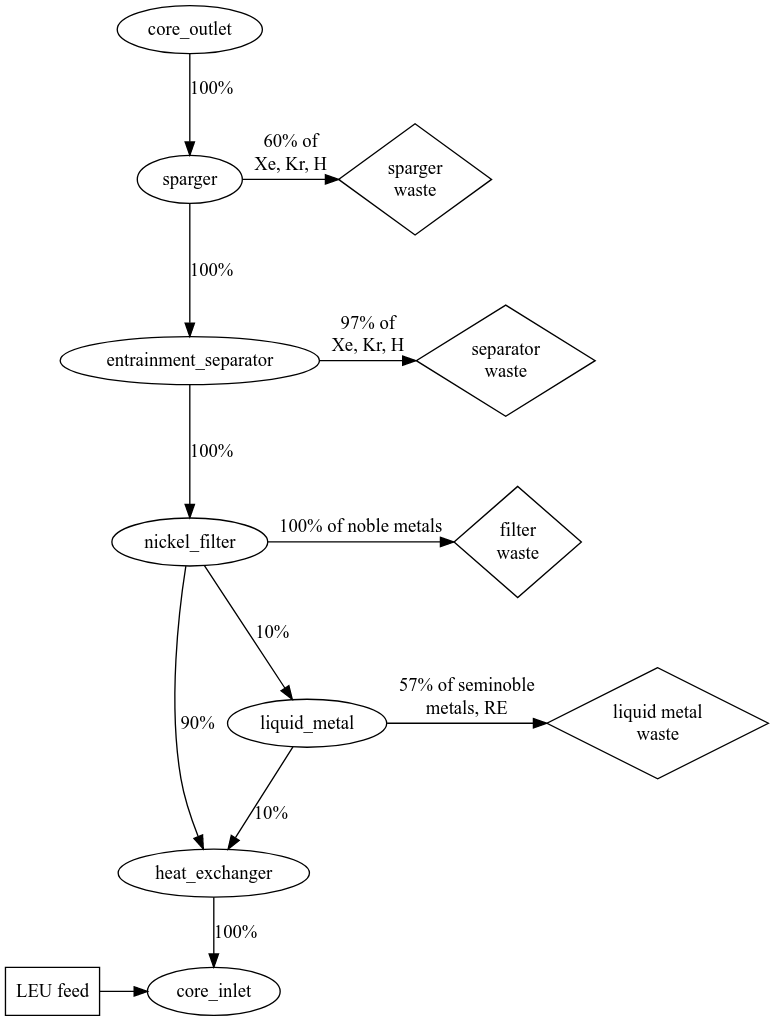
\includegraphics[width=0.93\textwidth]{demo_reprocessing_scheme.png}
	\caption{\gls{TAP} reprocessing scheme flowchart used for demonstration of 
	extended SaltProc. Arrows represent material flow; percents represent 
	fraction of total mass flow rates; ellipses represent fuel reprocessing 
		system components; diamonds represent waste streams; the box shows 
		refuel material flow.}
	\label{fig:demo-repro-scheme}
\end{figure}

The gas removal components (the sparger and entrainment separator) are located 
in-line because estimated full loop time for the fuel salt is about 18 seconds 
and approximately equal to the cycle time (table~\ref{tab:reprocessing_list}). 
To remove all volatile gases every 20 seconds, the gas removal system must 
operate with 100\% of the core throughout flow rate (in-line gas removal 
system). For the demonstration case herein to achieve required cycle time, the 
simulations herein assumed that xenon, krypton, and hydrogen extraction 
efficiencies for the sparger and entrainment separator are equal to 60\% and 
97\%, respectively.

The nickel filter in the \gls{TAP} concept is designed to extract noble metals 
and volatile fluorides. Similarly to volatile gases, noble metals must be 
removed every 20 seconds and, hence, the filter should operate in-line also. 
The nickel filter removes a wide range of elements with various efficiencies 
(table~\ref{tab:reprocessing_list}).

Lanthanides and other non-noble metals generally have a lower capture  
cross section and absorb fewer neutrons than gases and noble metals. These 
elements can be removed via a liquid-metal/molten salt extraction process with 
relatively low removal rates (cycle time $> 50$ days). This is accomplished 
by directing a small fraction of the salt mass flow leaving the nickel mesh 
filter (10\%). That fraction then flows to the liquid-metal/molten salt 
component of the reprocessing system, where lanthanides are removed with a 
specific extraction efficiency to match the  required cycle time 
(table~\ref{tab:reprocessing_list}). The rest 90\% of the salt mass flow is 
directed from the nickel filter to heat exchanger without performing any fuel 
salt treatment.

The removal rates vary among nuclides in this reactor concept, which dictate 
the necessary resolution of depletion calculations. To compromise, a 3-day 
time was selected based on timestep refinement study by Betzler \emph{et al.} 
\cite{betzler_assessment_2017}.
\subsection{Effective multiplication factor}
Figures~\ref{fig:keff}, \ref{fig:keff-zoomed}, and \ref{fig:keff-zoomed-2} 
demonstrate the effective multiplication factors obtained using SaltProc v1.0 
and Serpent. SaltProc obtained the effective multiplication factors after 
removing fission products and adding feed material at the end of each 
depletion step (3 days for this work). The $k_{eff}$ fluctuates significantly 
as a result of the batch-wise nature of this online reprocessing strategy.
\begin{figure}[htp!] % replace 't' with 'b' to 
	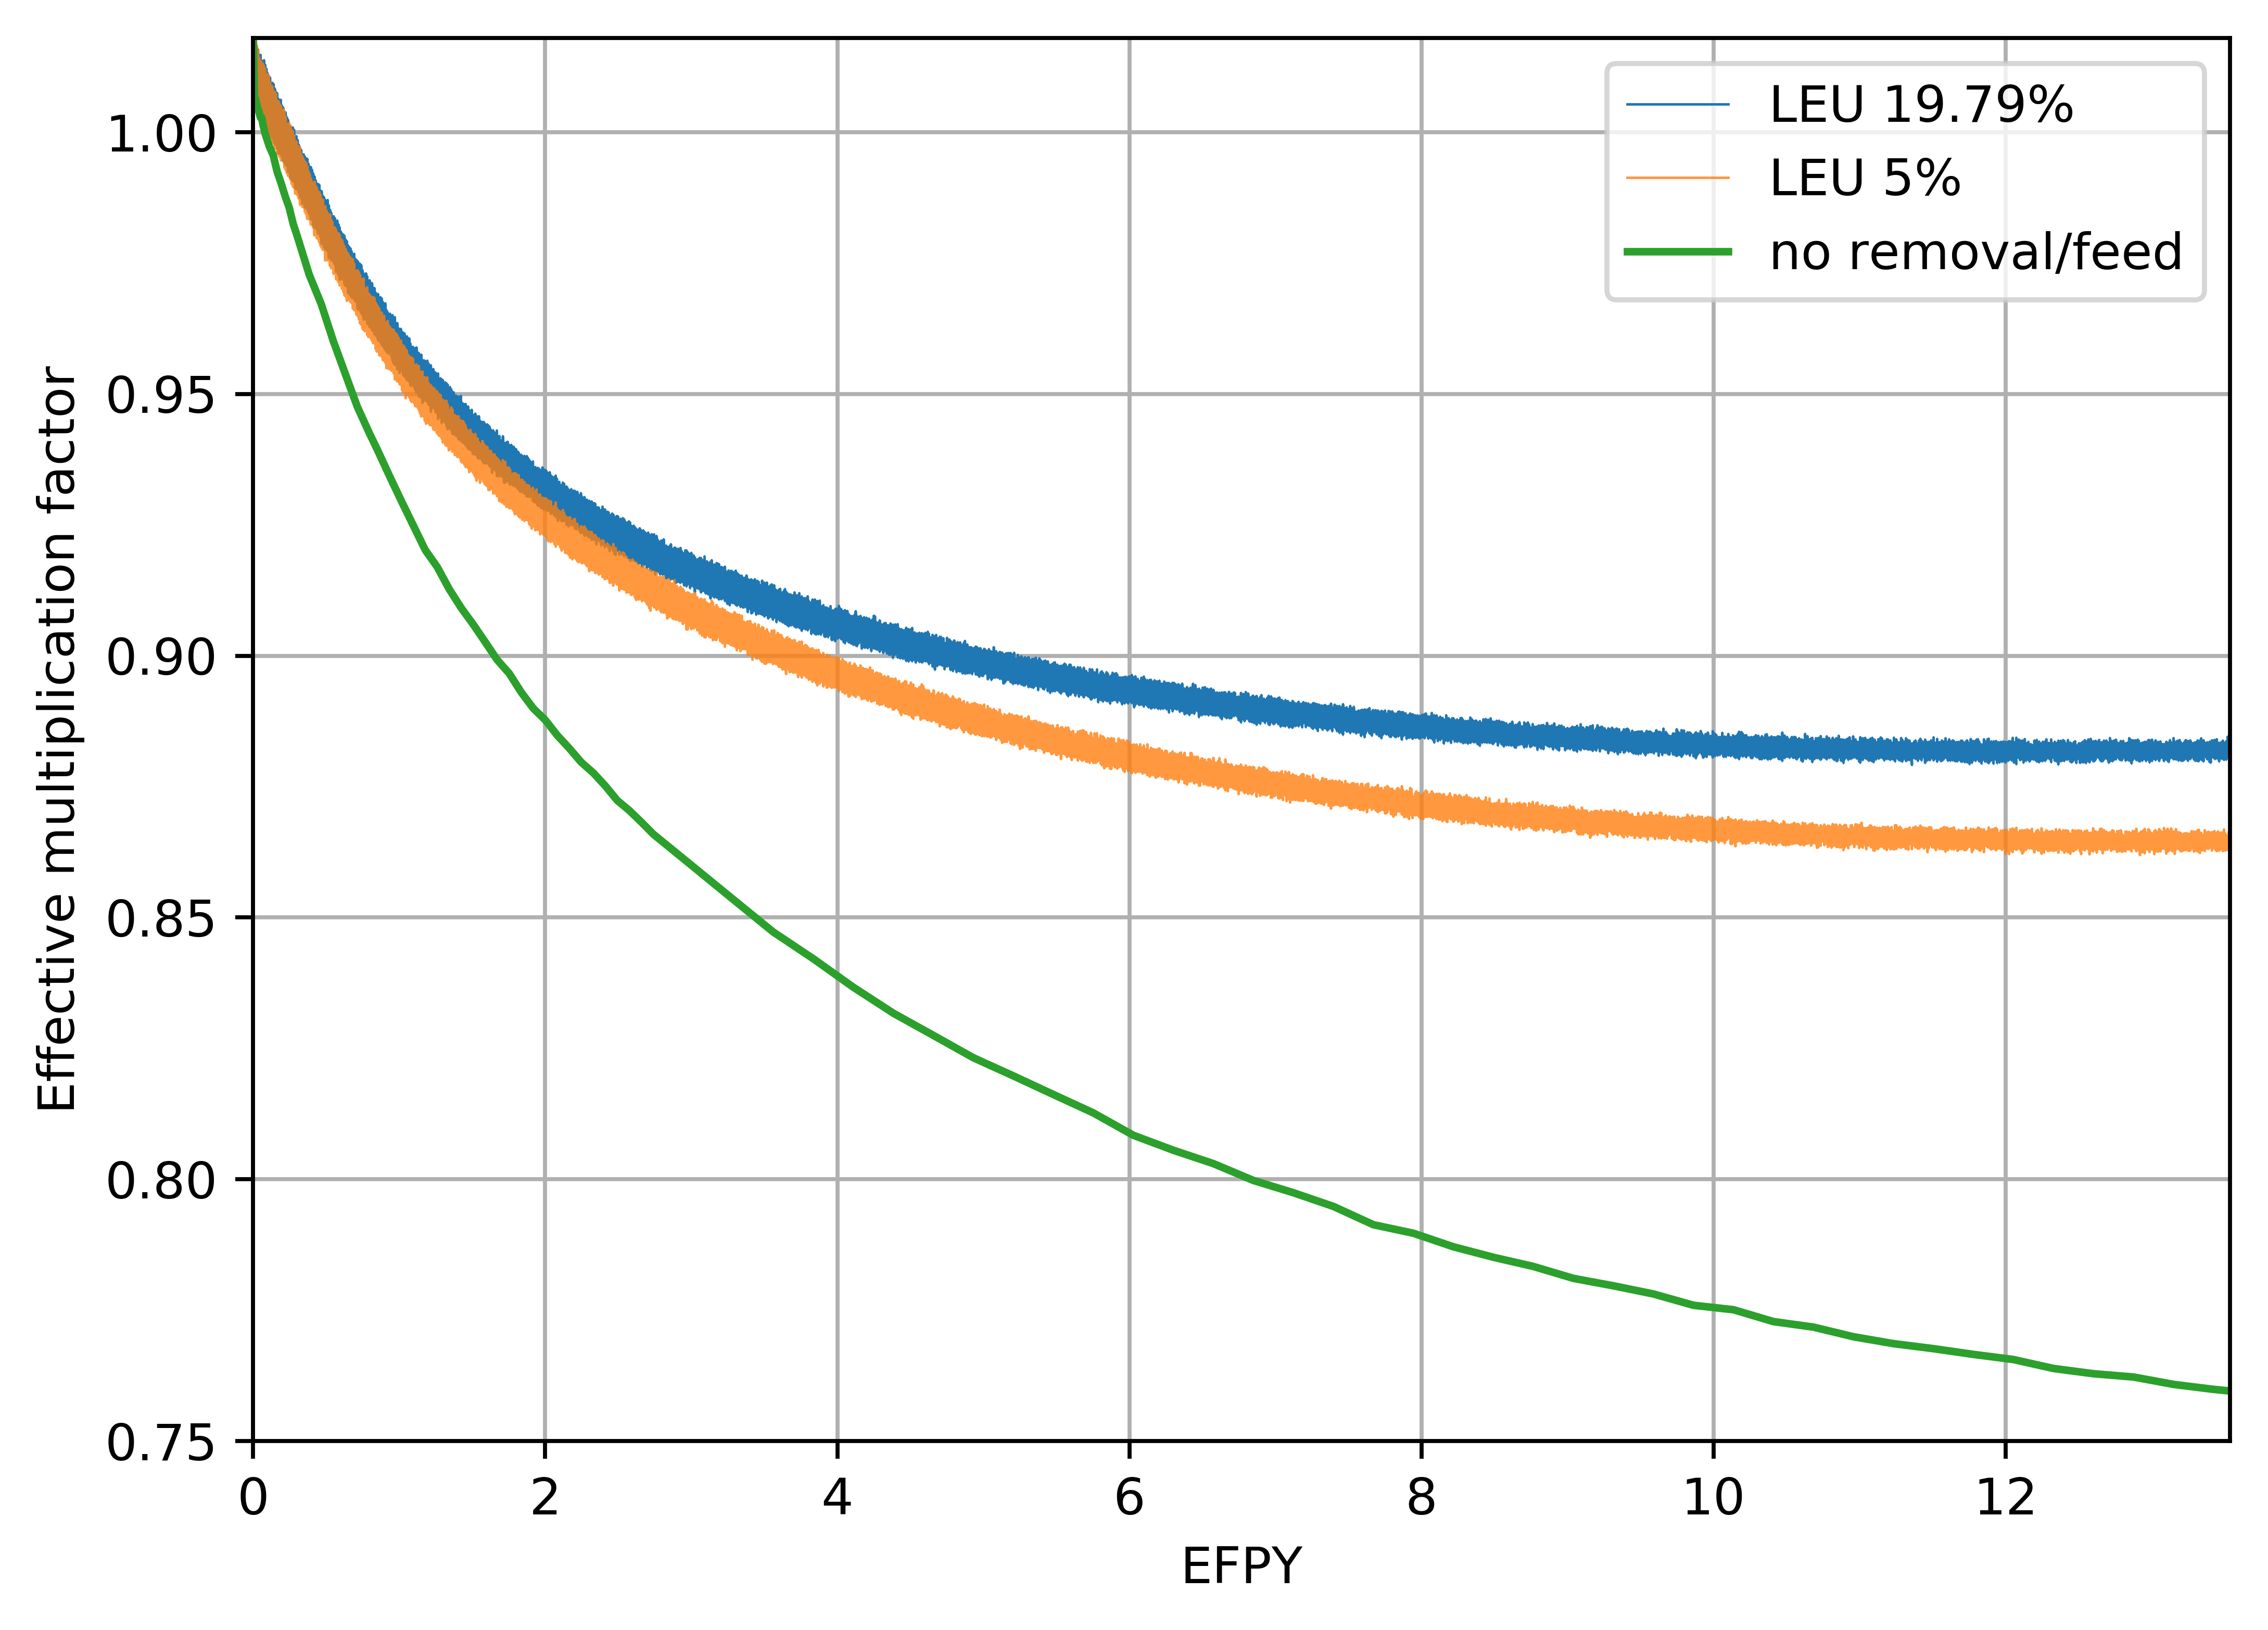
\includegraphics[width=\textwidth]{keff_3.png}
	\vspace{-0.2in}
	\caption{Effective multiplication factor dynamics for full-core
		\gls{TAP} model for different fueling scenarios over a 13-year reactor 
		operation. 
		Confidence interval $\pm\sigma=28pcm$ is shaded.}
	\label{fig:keff}
\end{figure}
\begin{figure}[htp!] % replace 't' with 'b' to 
	\centering
	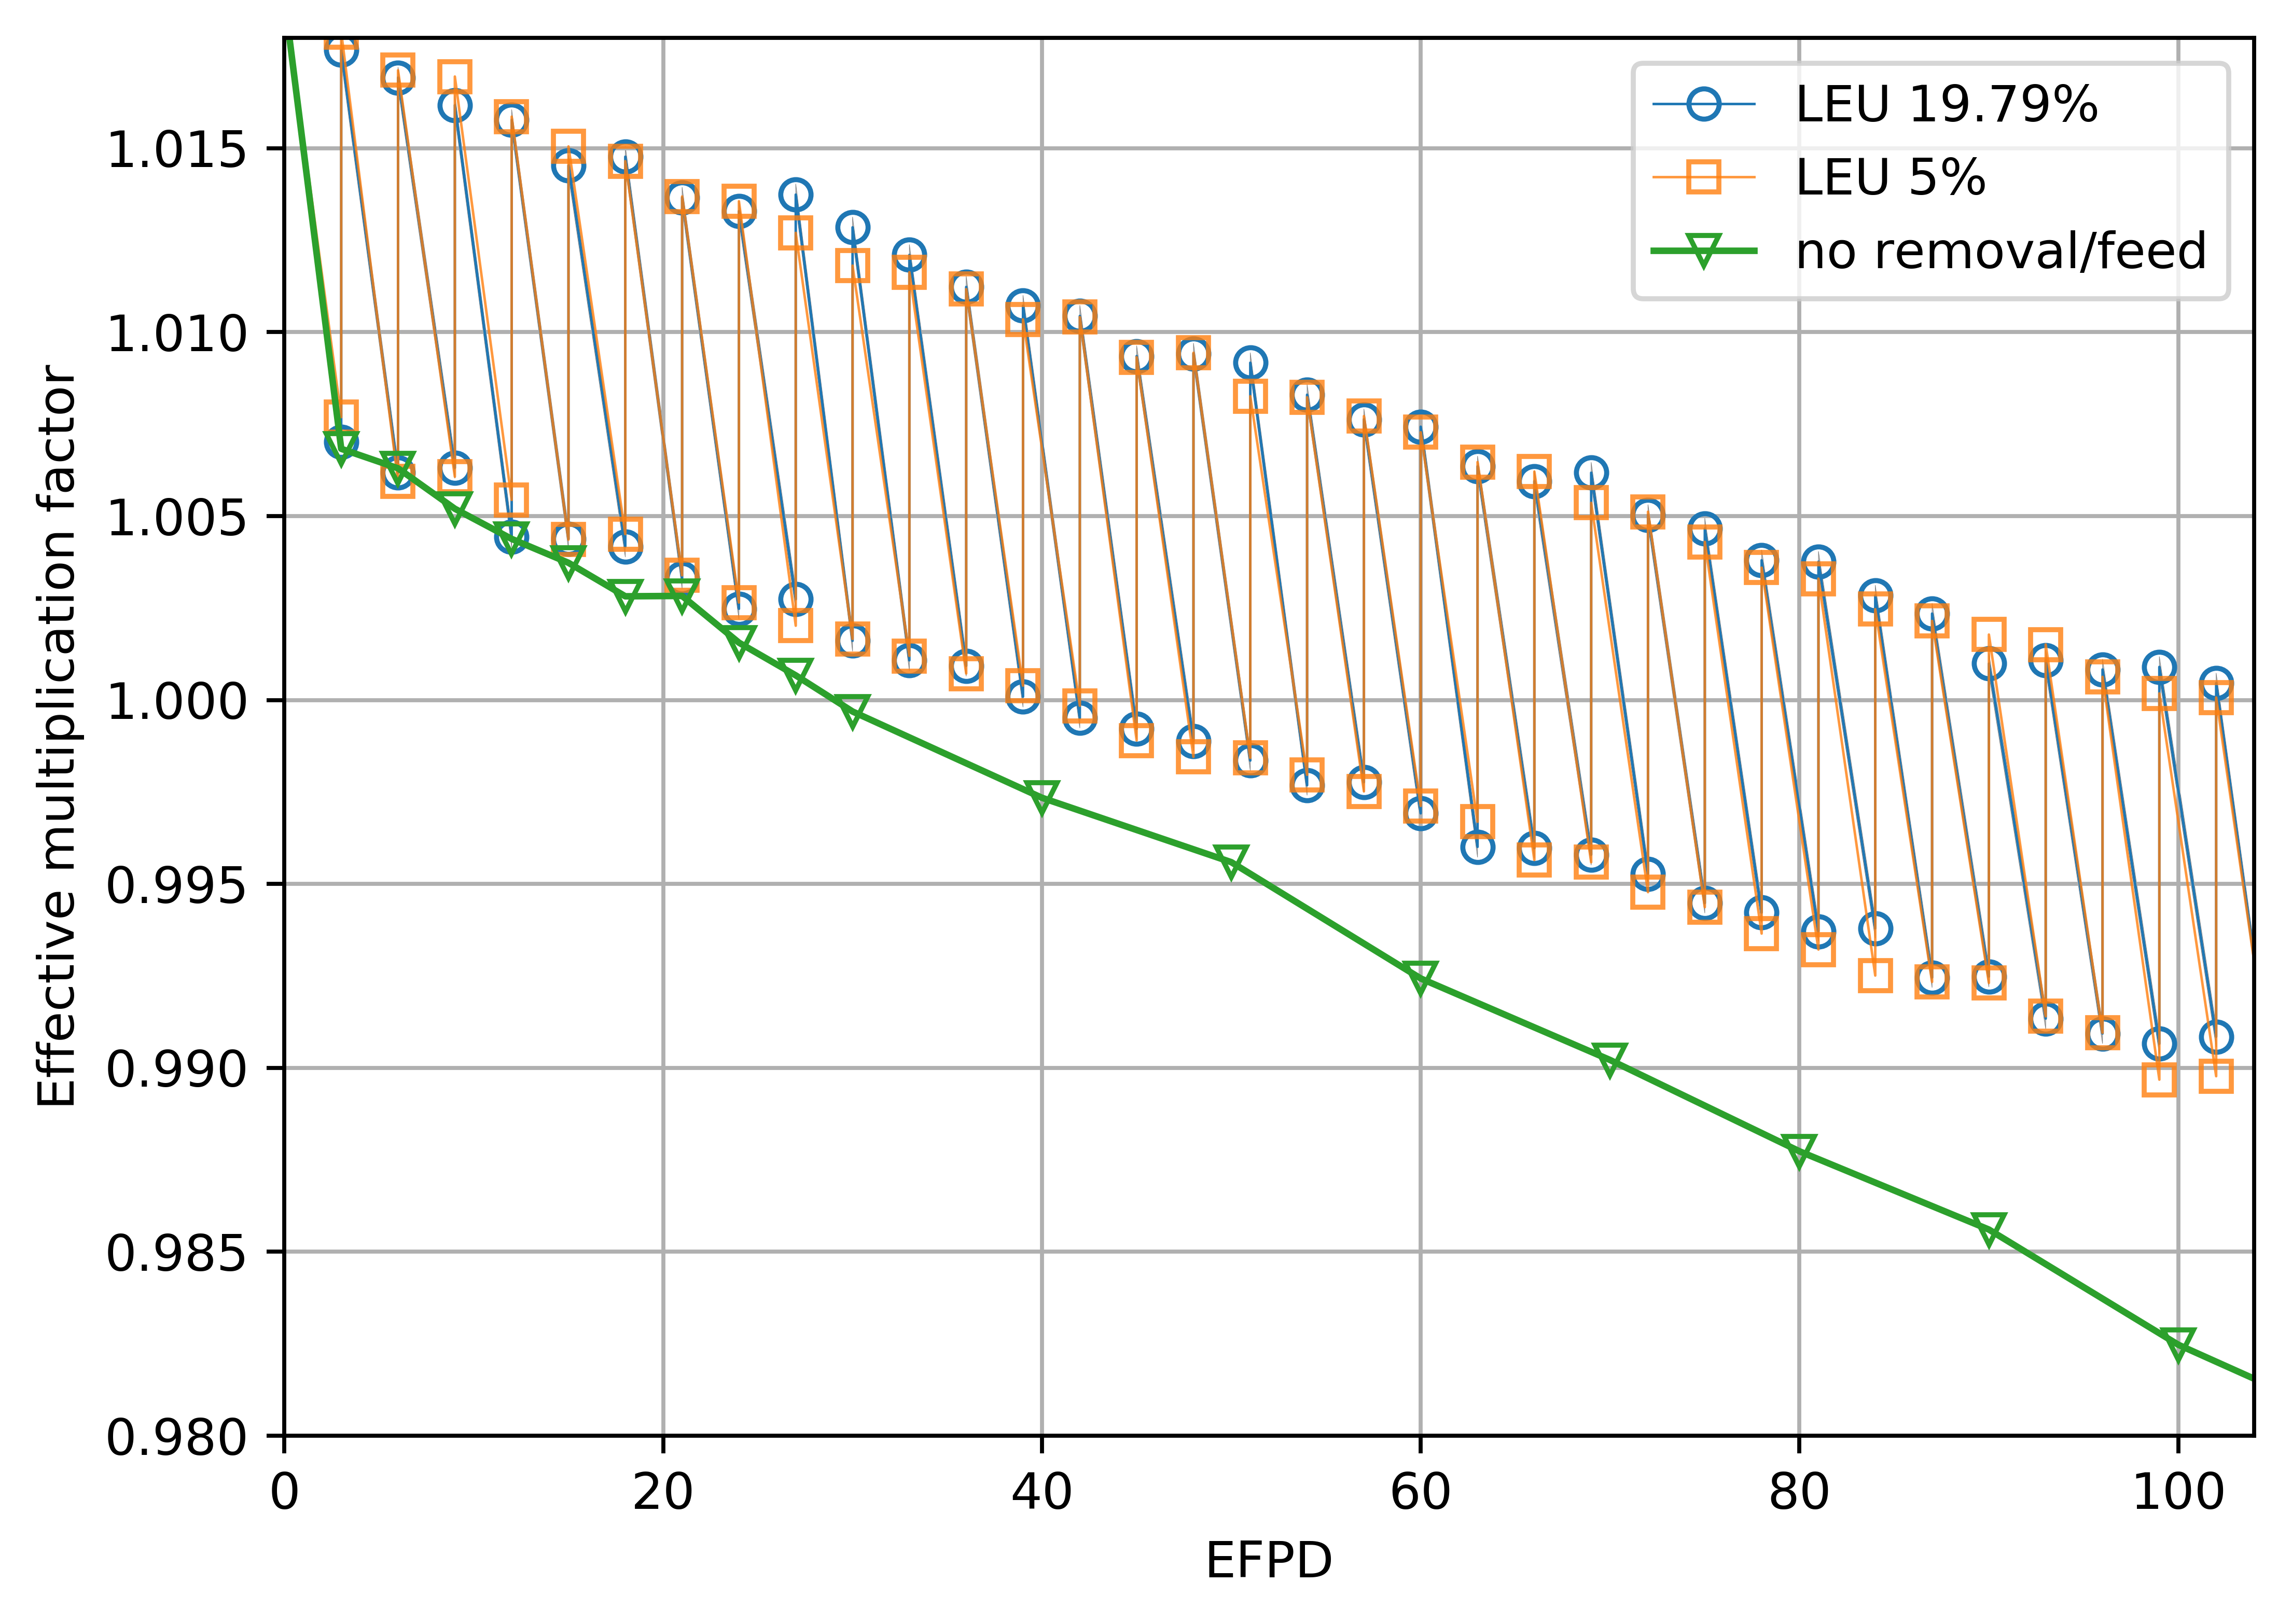
\includegraphics[width=0.85\textwidth]{keff_zoomed_1.png}
	\caption{Zoomed effective multiplication factor for the first 104 EFPD 
		after startup.}
	\label{fig:keff-zoomed}
\end{figure}
\begin{figure}[htp!] % replace 't' with 'b' to 
	\centering
	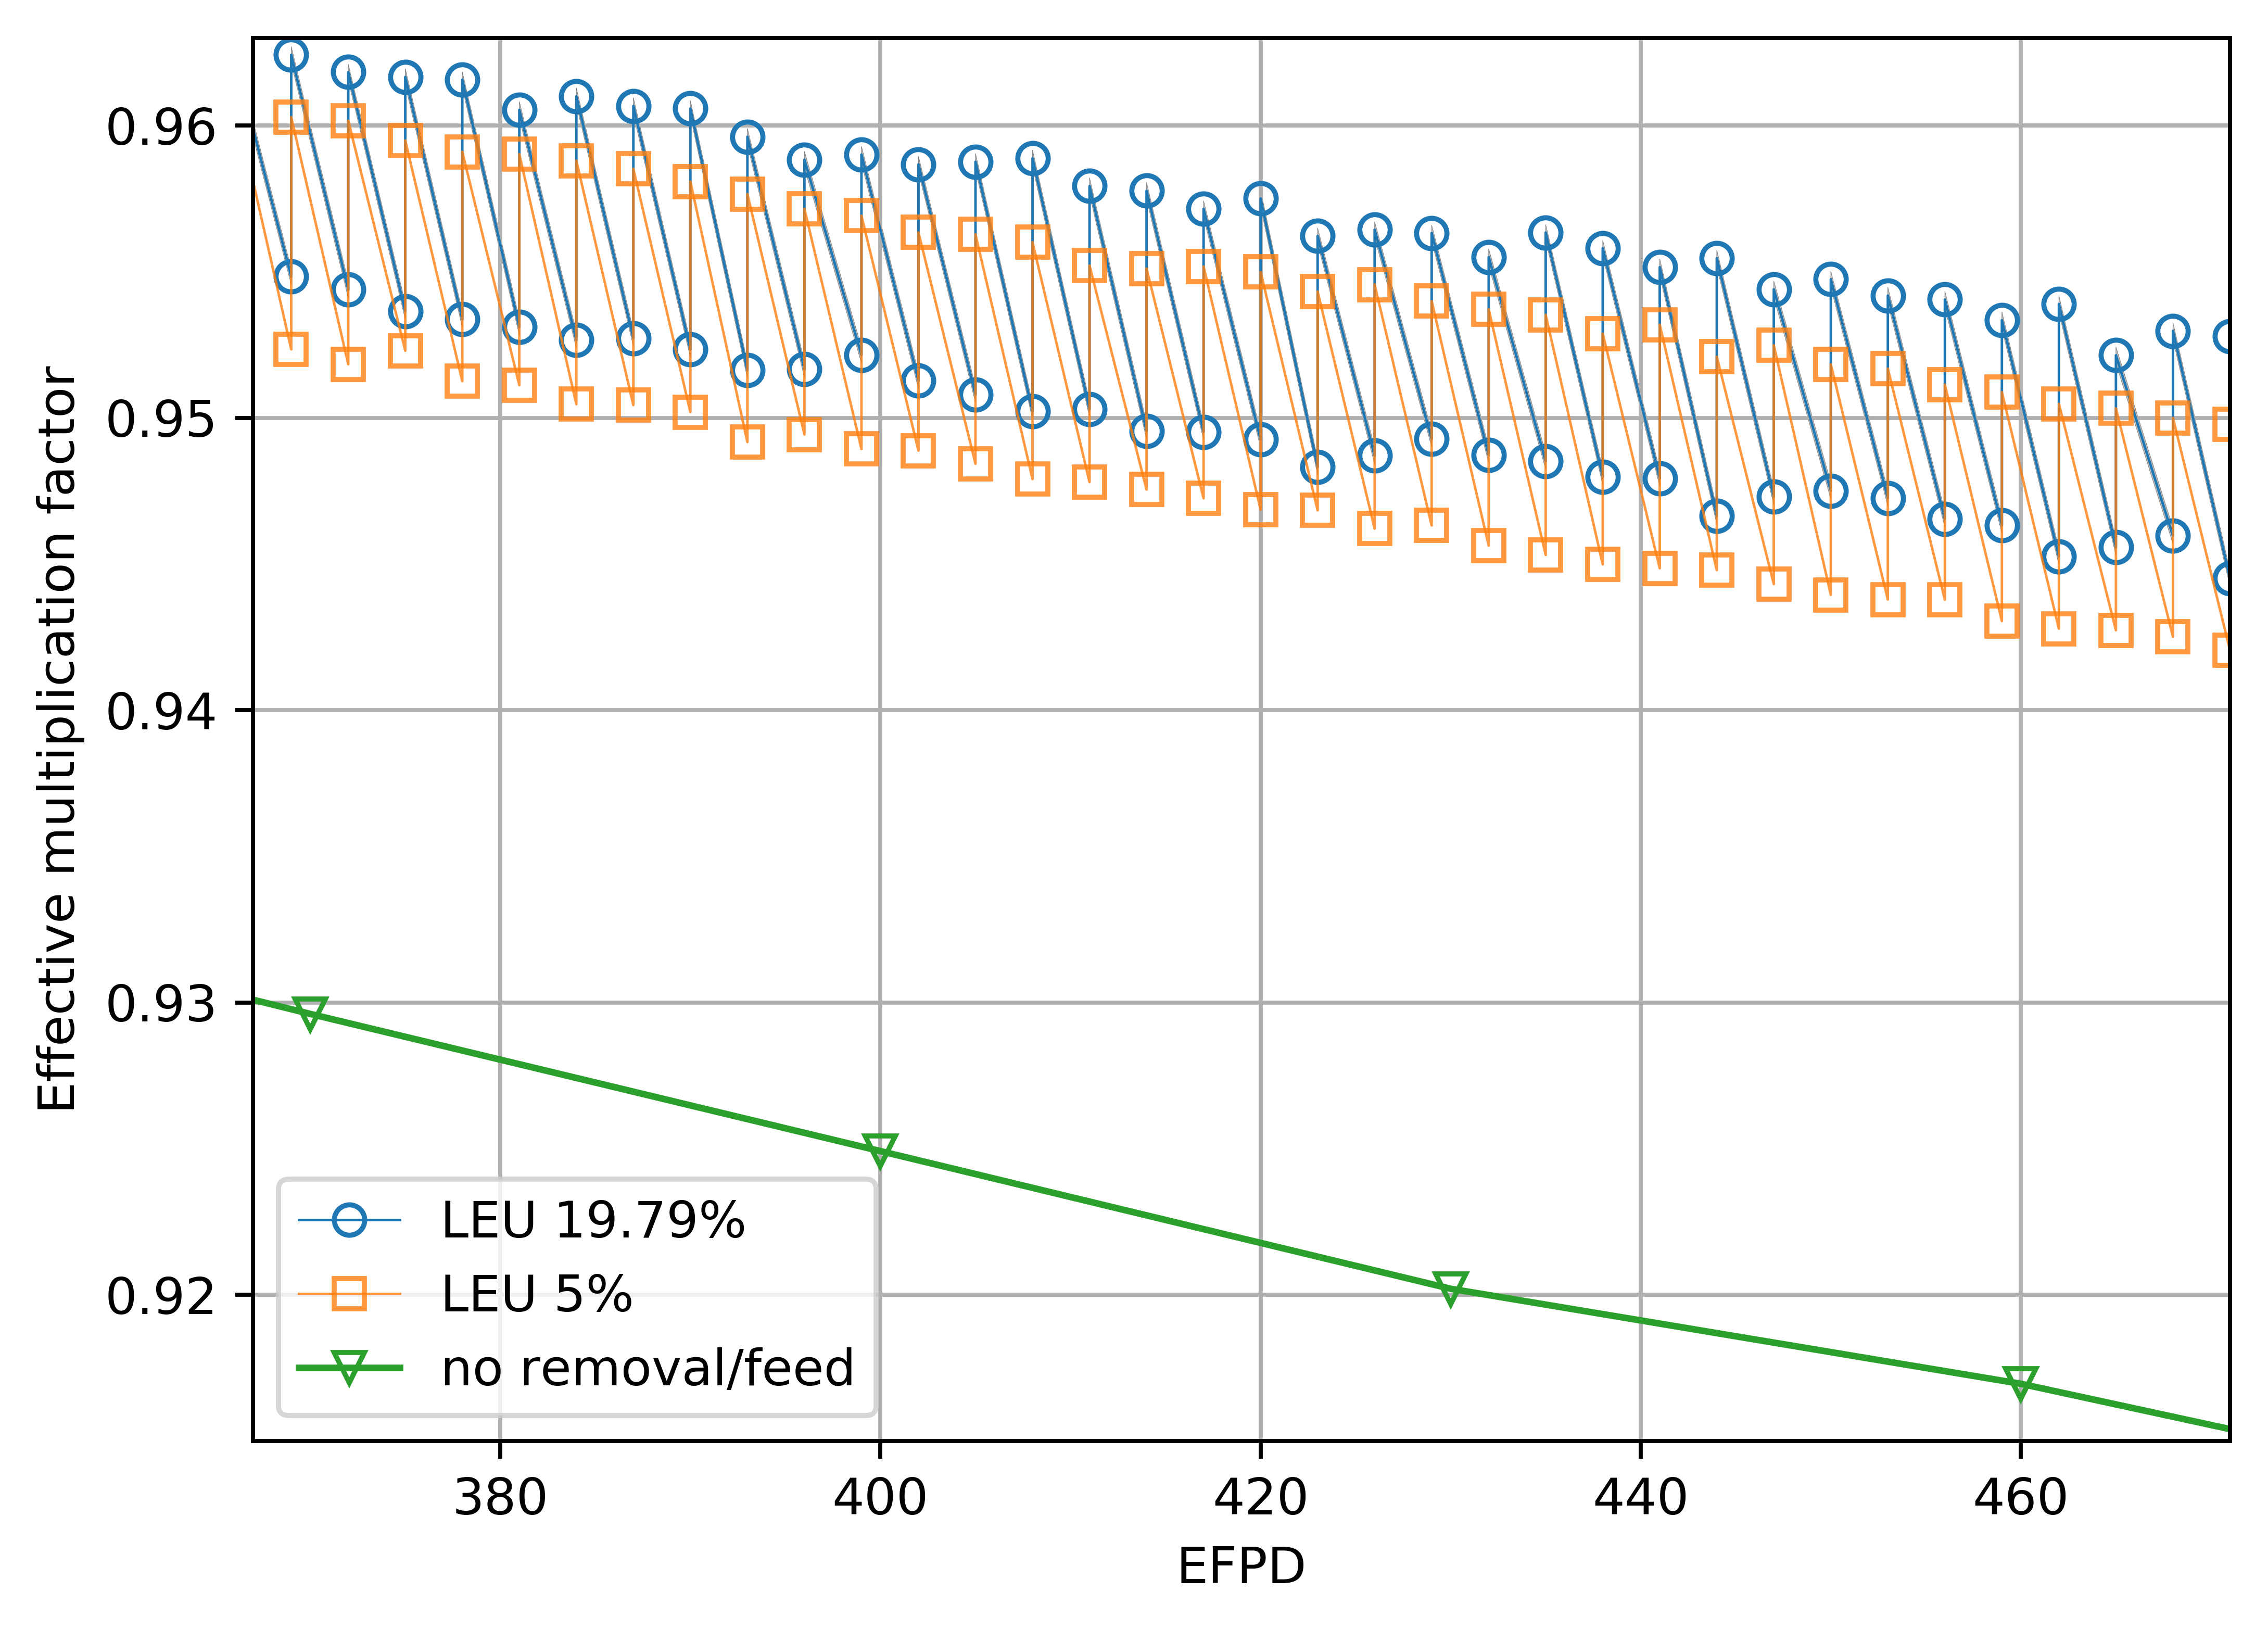
\includegraphics[width=0.85\textwidth]{keff_zoomed_2.png}
	\caption{Zoomed effective multiplication factor for the time interval 
		from 367 to 471 EFPD after startup.}
	\label{fig:keff-zoomed-2}
\end{figure}

Loading initial fuel salt composition with 5\% \gls{LEU} into the \gls{TAP} 
core leads to a supercritical configuration with an excess of reactivity about 
1900pcm (figure~\ref{fig:keff}). Without performing any fuel salt reprocessing 
the core became subcritical after 30 days of operation  
(figure~\ref{fig:keff-zoomed}). I obtained this result using Serpent on its 
own, without introducing any \gls{FP} extraction and refueling. For the 
beginning of the \gls{TAP} reactor lifetime, uranium enrichment in the feed 
has a minor effect because a tiny amount of poisons was produced ($<$1kg/day) 
and, hence, a small mass of fresh salt was injected. Notably, the core went 
subcritical after 42 days of operation either with \gls{LEU} 5\% or \gls{LEU} 
19.79\% feed.

The \gls{TAP} core is never reached equilibrium fuel salt composition without 
performing fuel salt reprocessing and refueling. For the fueling scenarios 
with 5\% and 19.79\% \gls{LEU} feed, the reactor achieved the equilibrium 
state after 10 years of operation. Overall, the effective multiplication 
factor gradually decreases from 1.018 to 0.88 for the 19.79\% \gls{LEU} feed 
and 0.86 for the 5\% \gls{LEU} feed, which indicates problems with operating 
this nuclear reactor design. The proposed continuation of this work will to 
overcome this issue by adding dynamic \gls{SVF} functionality to SaltProc v1.0.

\subsection{Neutron spectrum}
Figure~\ref{fig:spectrum} shows the normalized neutron flux spectrum for the 
full-core \gls{TAP} core model in the energy range from 10$^{-8}$ to 15 MeV. 
The neutron energy spectrum at equilibrium is slightly harder than at 
startup due to plutonium and other strong absorbers accumulating in the 
core during reactor operation. The \gls{TAP} reactor spectrum is significantly 
harder than in a typical \gls{LWR} and is in a good agreement with 
\gls{ORNL} report \cite{betzler_assessment_2017}.
\begin{figure}[htp!] % replace 't' with 'b' to 
	\centering
	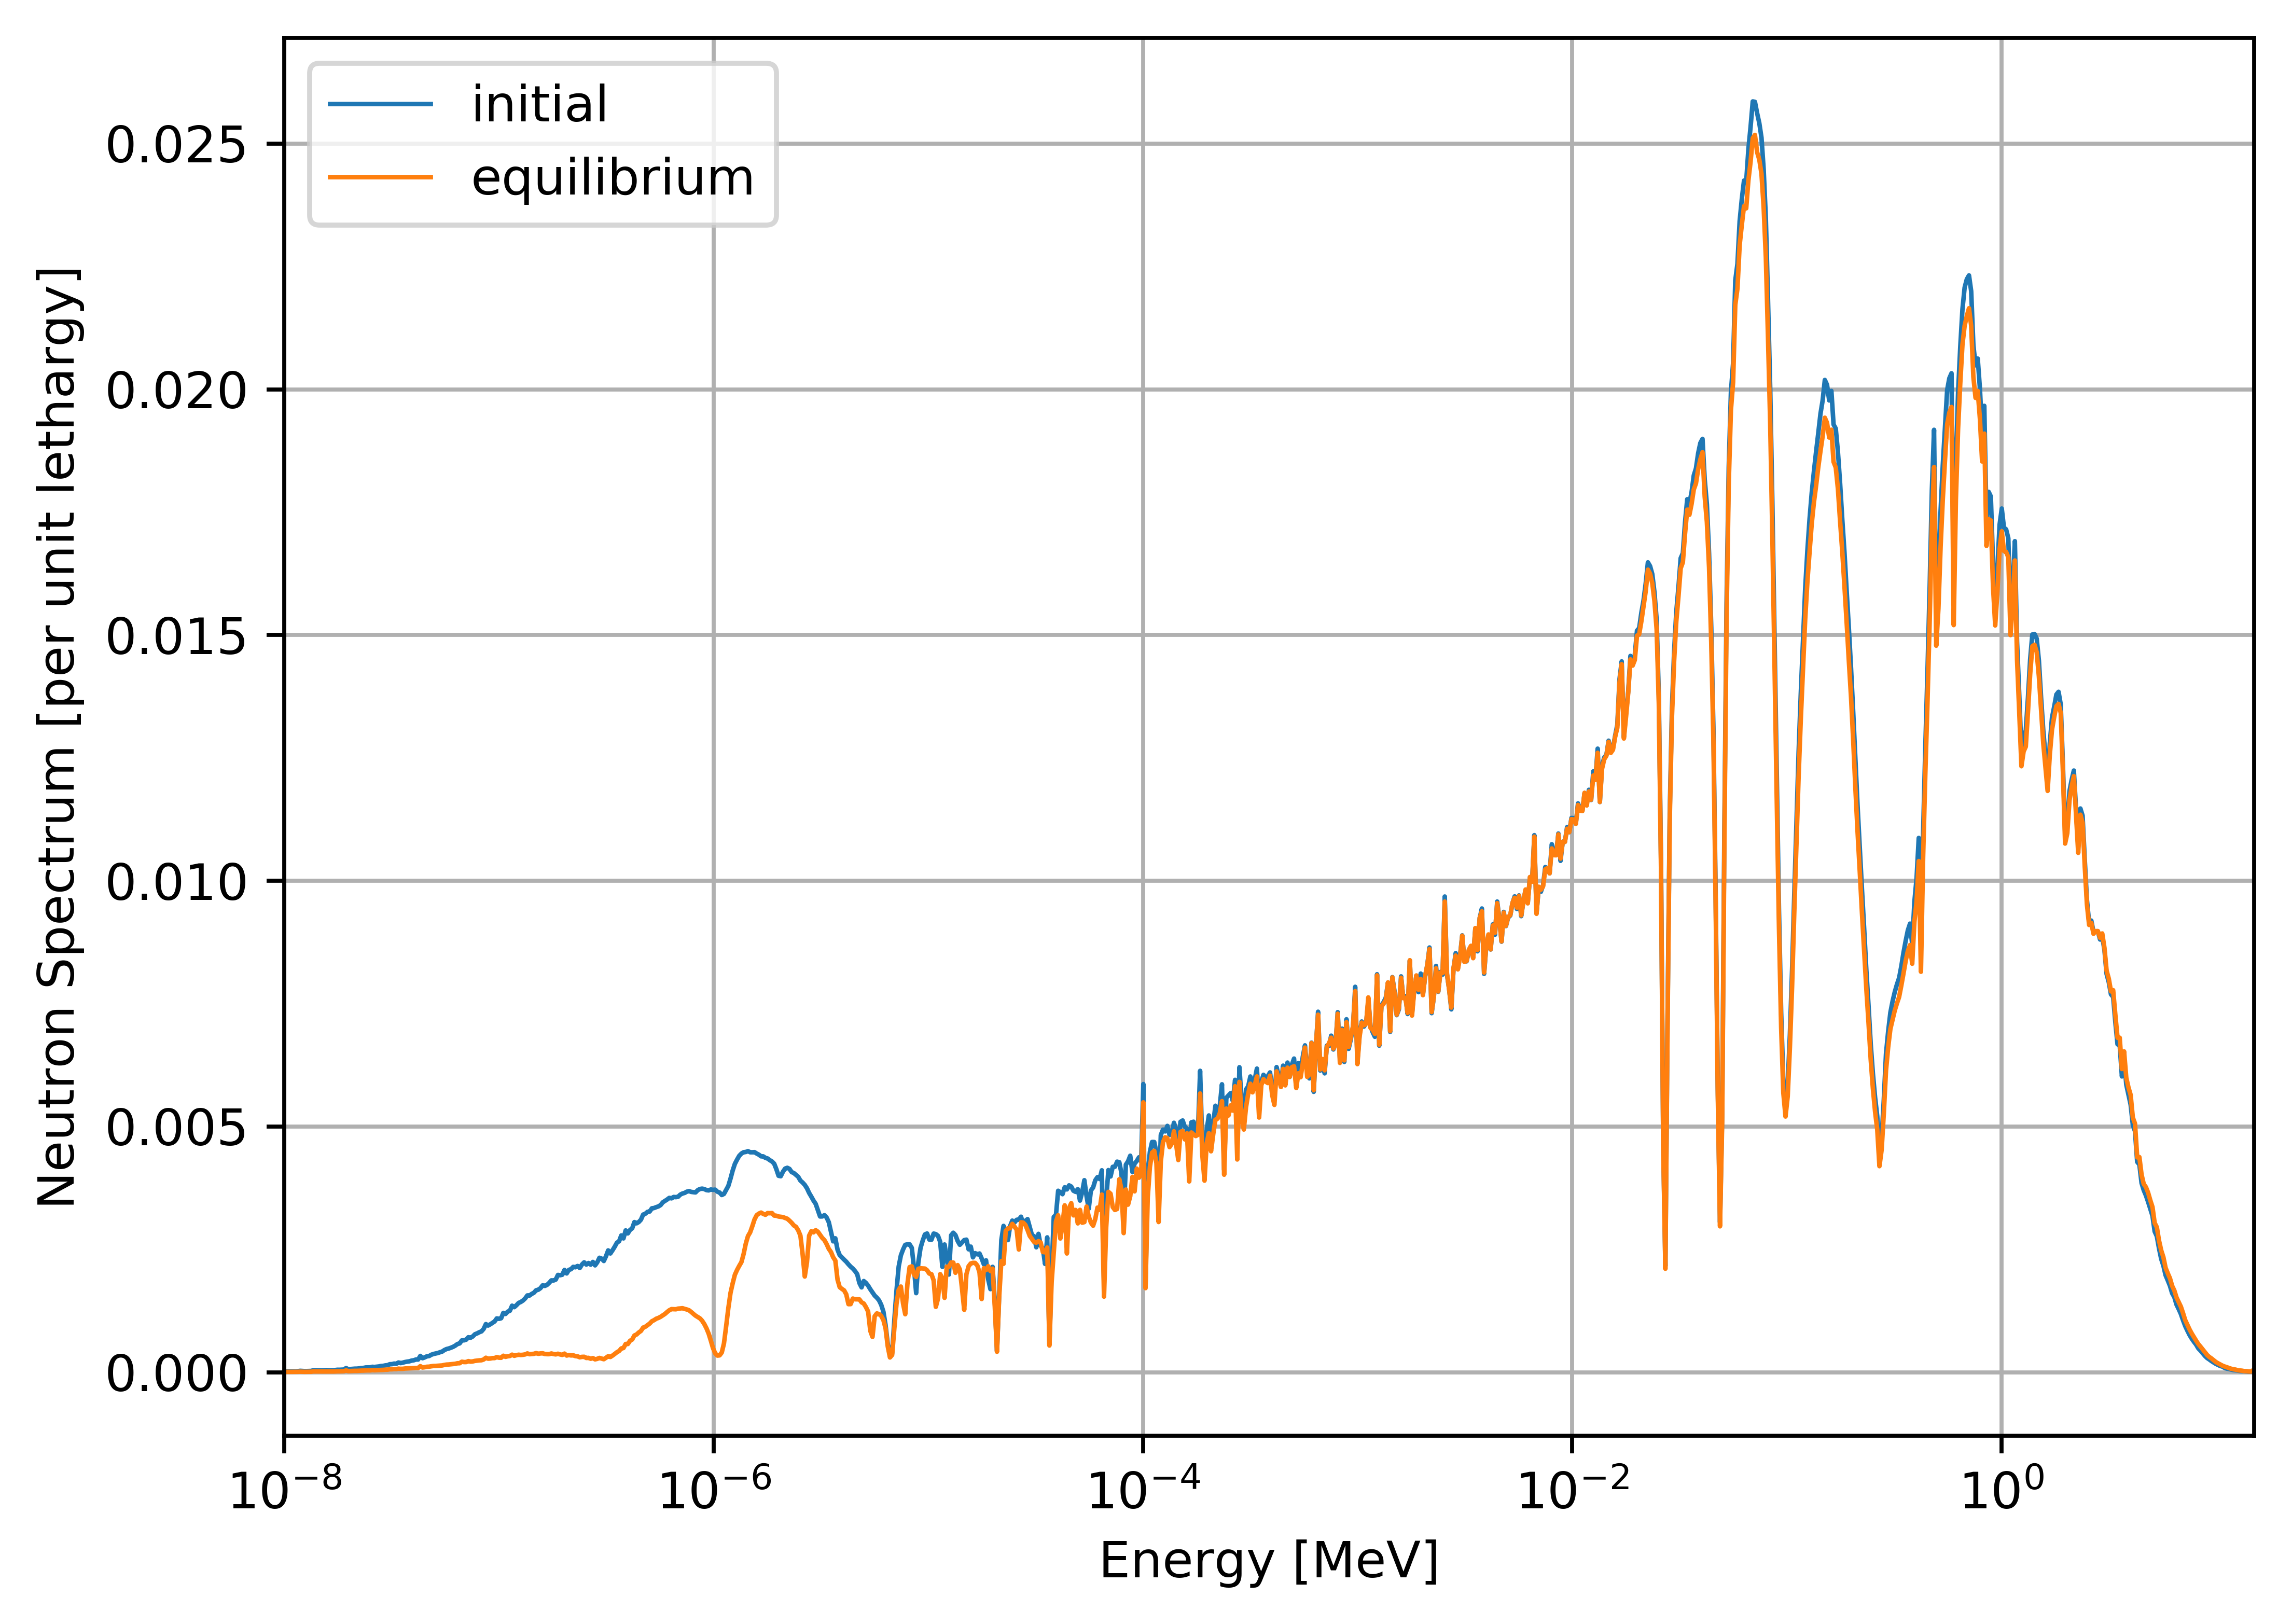
\includegraphics[width=\textwidth]{spectrum.png}
	\caption{The neutron flux energy spectrum normalized by unit lethargy 
		for initial and equilibrium fuel salt composition.}
	\label{fig:spectrum}
\end{figure}
\subsection{Fuel salt composition}
Figure~\ref{fig:u-pu} shows the absolute mass of major heavy isotopes 
which have a strong influence on the reactor core physics. The masses of 
$^{236}$U, $^{238}$U, $^{239}$Pu, $^{240}$Pu, and $^{241}$Pu in the 
fuel salt change insignificantly after approximately 10 years of operation,
which matches the stabilization time for the effective multiplication factor. 
Hence, the quasi-equilibrium state was reached after 10 years of reactor 
operation. Moreover, the \gls{TAP} core bred approximately the same amount 
of fissile $^{239}$Pu ($\approx2$t) as corresponds to the initial fissile 
material ($^{235}$U) load. A significant amount of non-fissile plutonium 
builds up during operation and accounts for 50\% of the plutonium after 13 
years of operation. Overall, the rate of breeding fissile $^{239}$Pu from 
$^{238}$U even in this relatively hard neutron spectrum is not large enough to 
compensate for the negative effects of strong absorber accumulation or to keep 
the reactor critical.
\begin{figure}[htp!] % replace 't' with 'b' to 
	\centering
	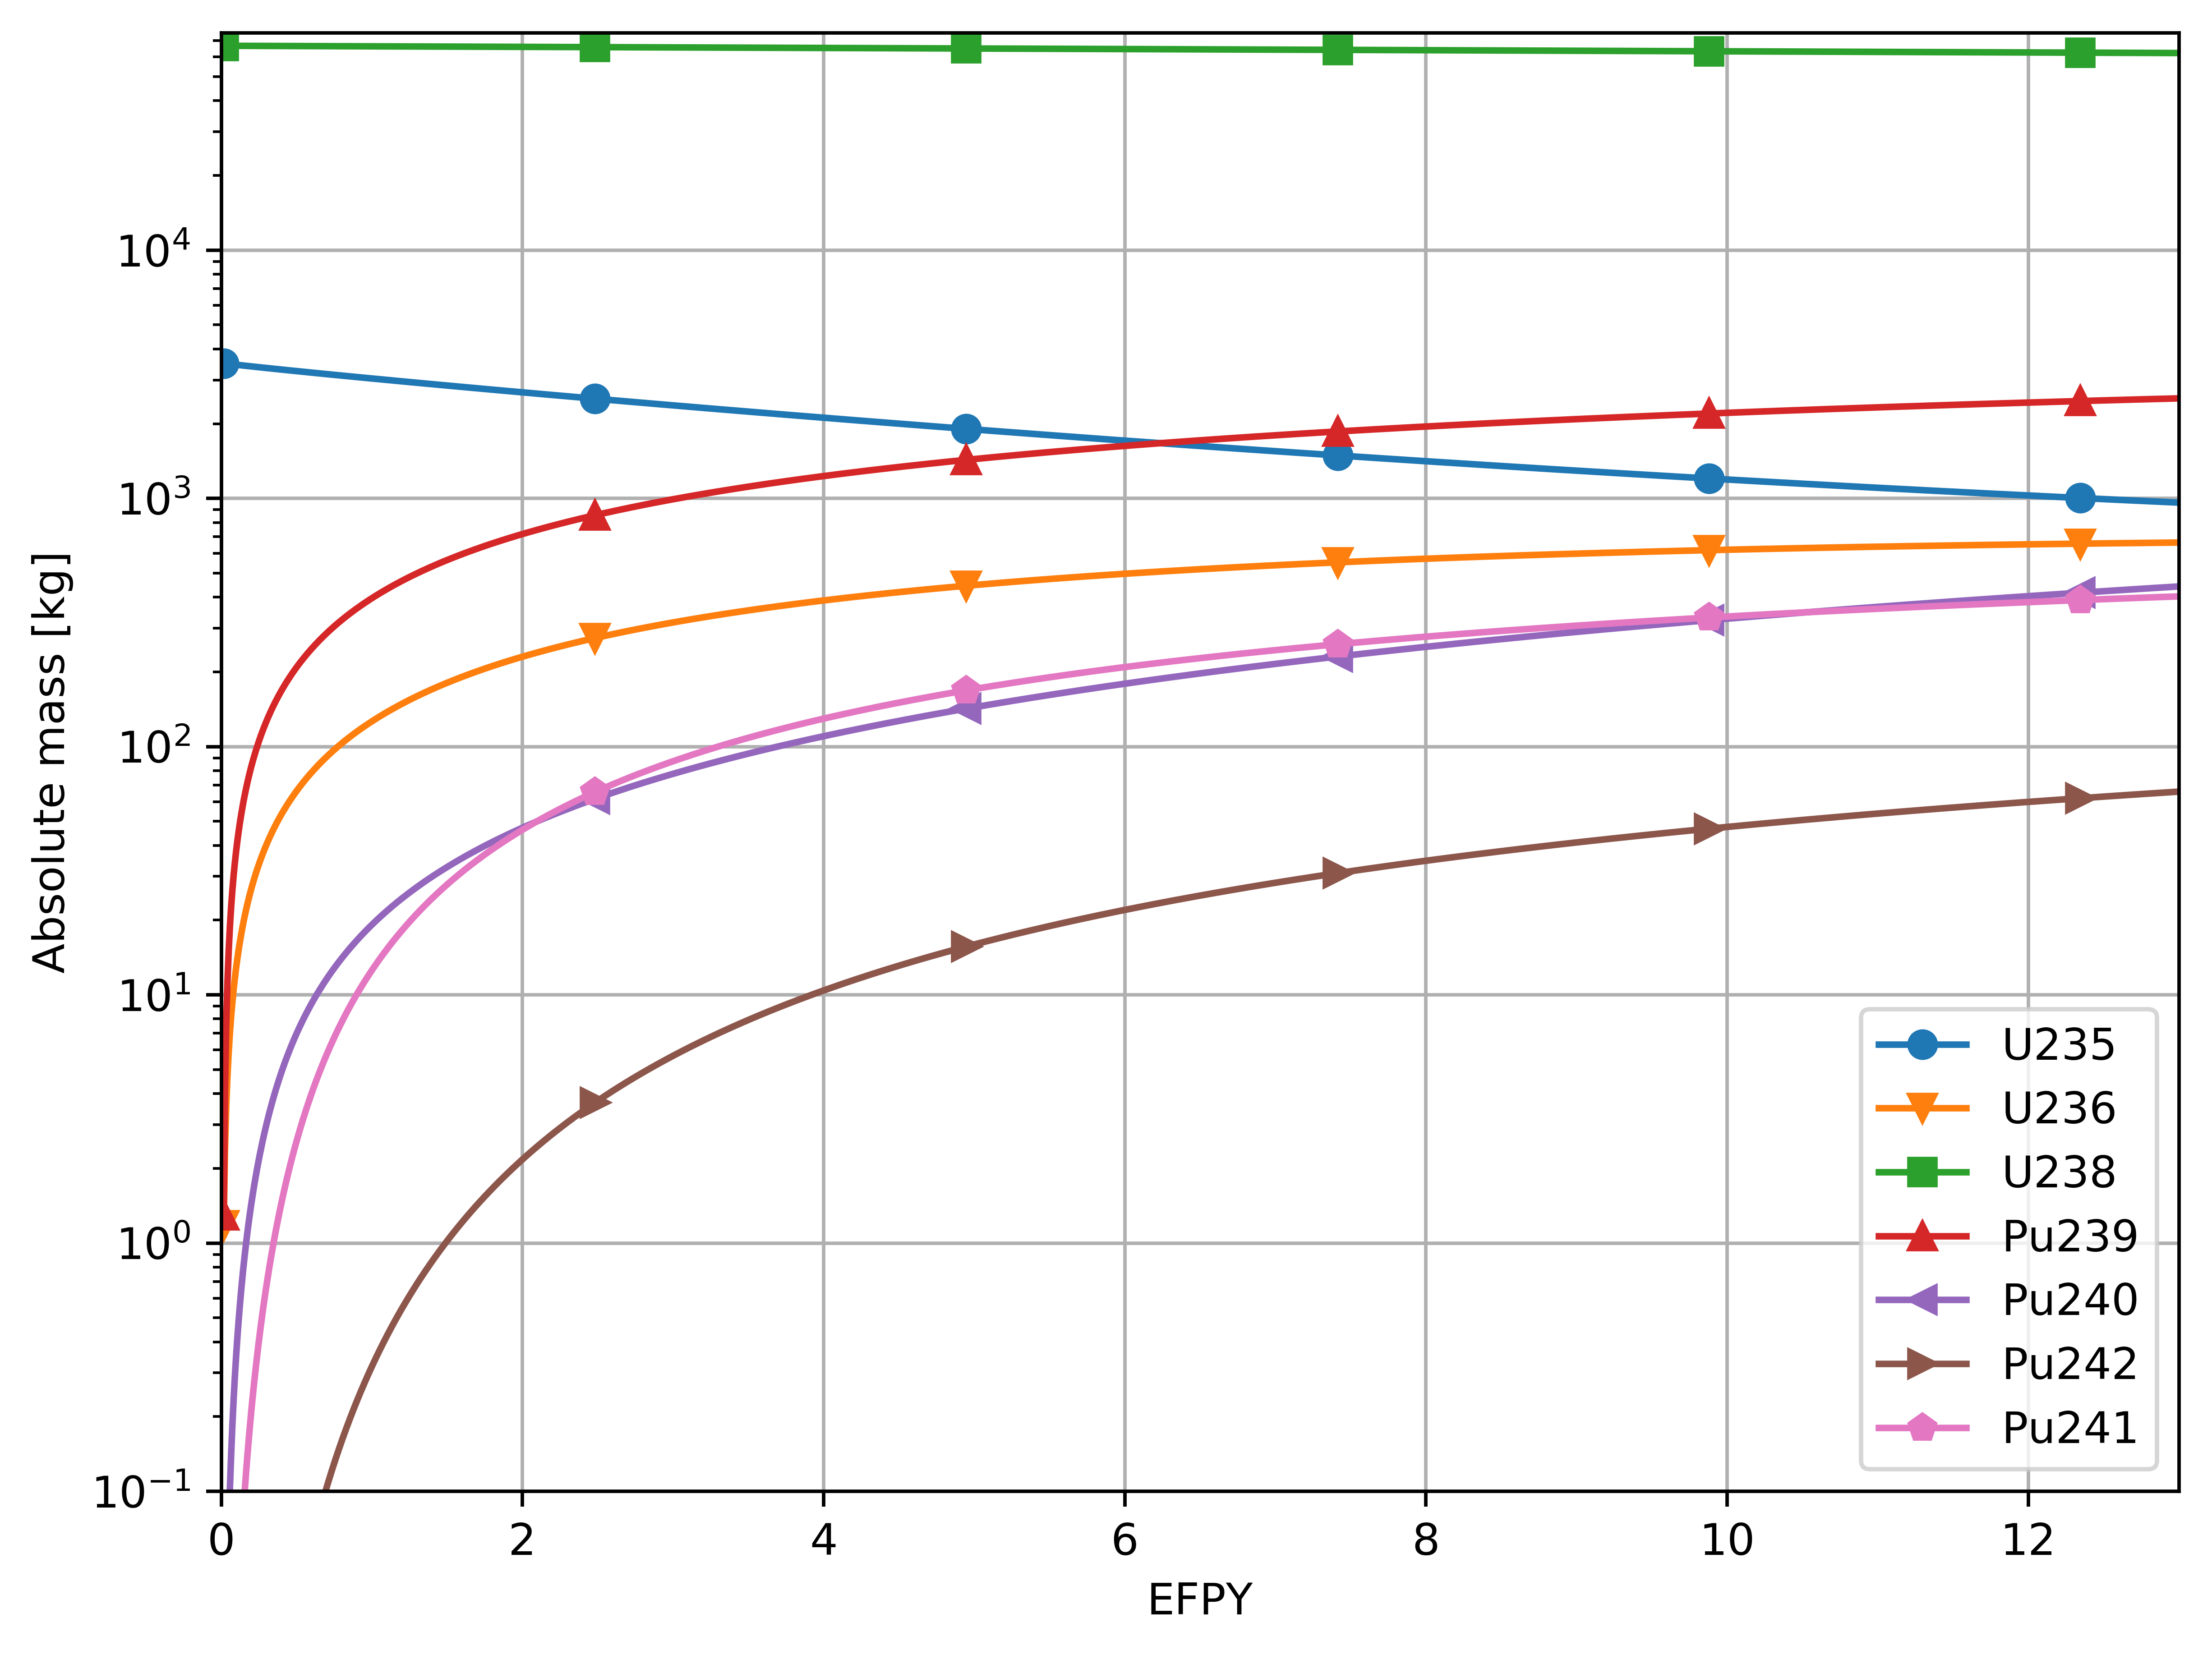
\includegraphics[width=\textwidth]{u_pu_mass.png}
	\caption{Mass of major nuclides during 13 years of reactor operation 
		with 19.79\% \gls{LEU} feed.}
	\label{fig:u-pu}
\end{figure}

I checked correctness of SaltProc v1.0 by comparing the masses of important 
isotopes for load-following operation ($^{135}$Xe, $^{135}$I) to the expected 
masses after each depletion step (figure~\ref{fig:xe-i}). For $^{135}$Xe, the 
expected mass was calculated as follows:
\begin{align}
\qquad\qquad\qquad & m_{post} = m_{pre} \times  
(1-\epsilon_{s}) \times (1-\epsilon_{es})
\intertext{where}
m_{post} &= \mbox{mass of the isotope after applying removals and feeds} 
\nonumber \\
m_{pre} &= \mbox{mass of the isotope right before  reprocessing} 
\nonumber \\
\epsilon_{s} &= \mbox{sparger extraction efficiency} \nonumber \\
\epsilon_{es} &= \mbox{entrainment separator extraction efficiency.} 
\nonumber
\end{align}
\begin{figure}[htp!] % replace 't' with 'b' to 
	\centering
	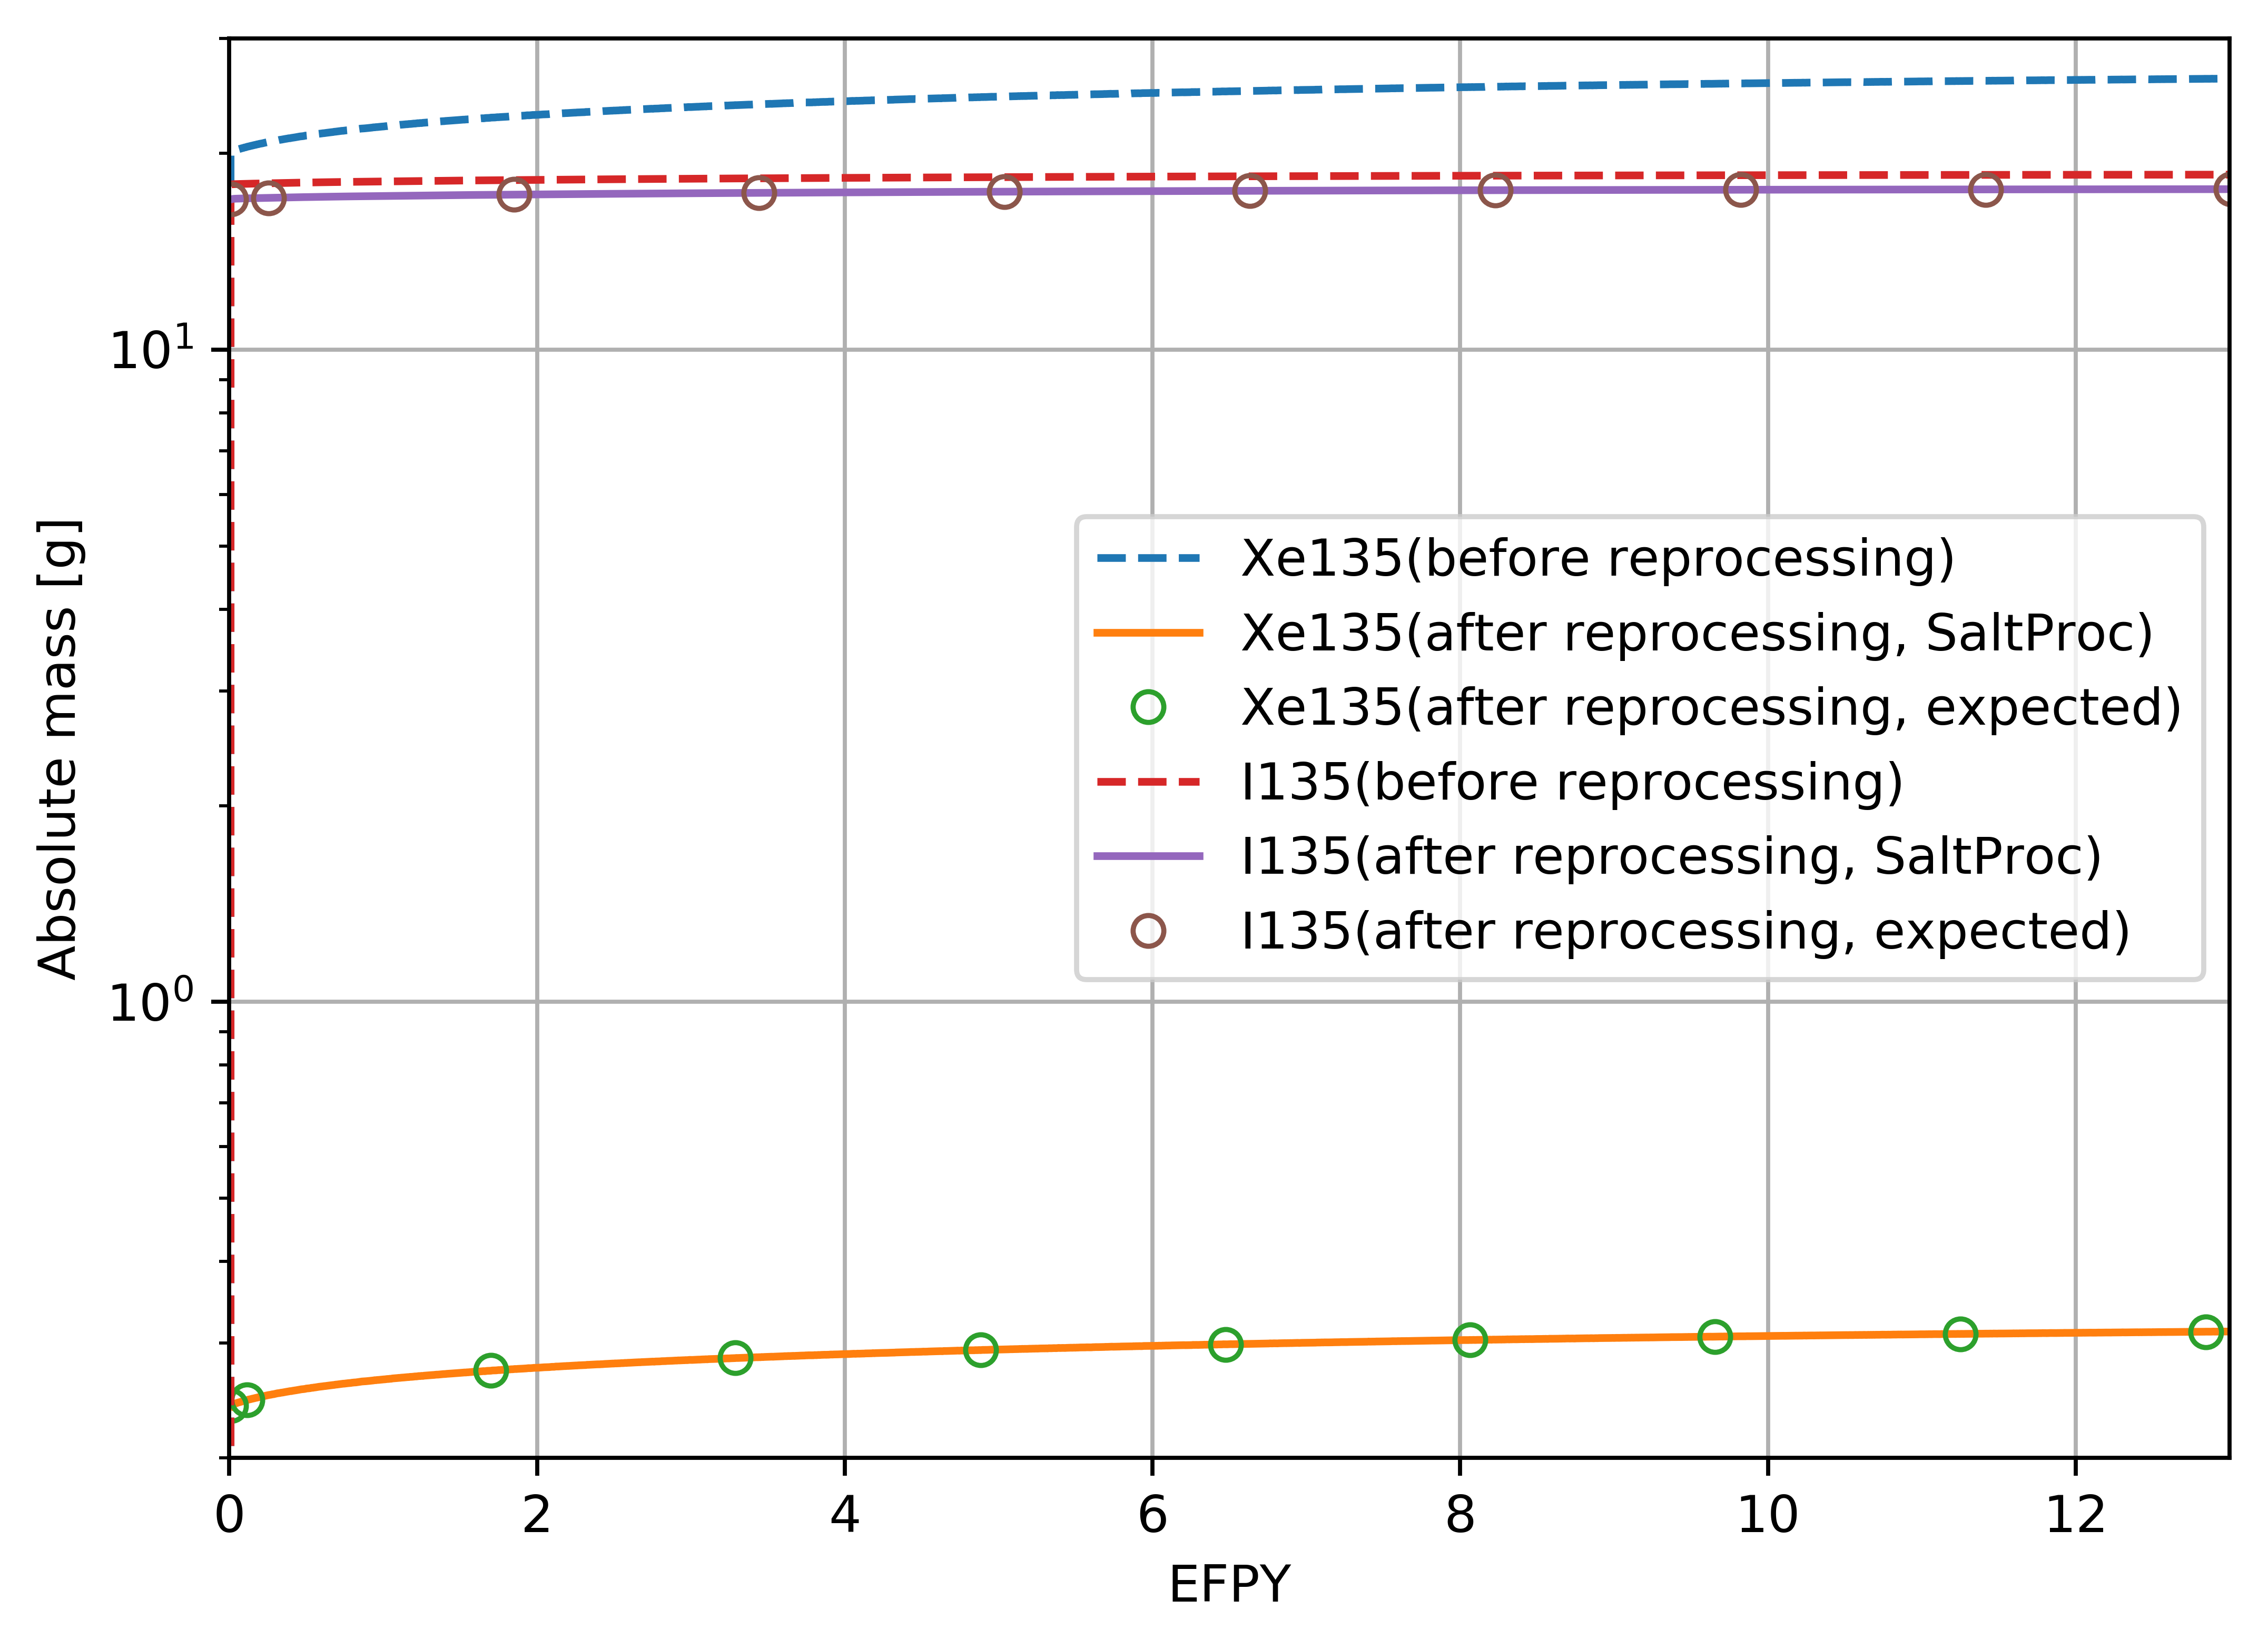
\includegraphics[width=0.95\textwidth]{xe_i_mass.png}
	\caption{Mass of major neutron poison, $^{135}$Xe, and its main precursor, 
		$^{135}$I, during 13 years of reactor operation before and after 
		performing reprocessing in SaltProc v1.0.}
	\label{fig:xe-i}
\end{figure}

For iodine, the approach is similar, but the extraction efficiency of iodine 
in the nickel filter is only 5\%. Figure~\ref{fig:xe-i} shows that SaltProc 
v1.0 extraction module correctly removes target isotopes with specified 
extraction efficiency: SaltProc calculations match the expected mass.
